\documentclass[10pt, letterpaper]{report}
% !TeX program = xelatex
%==================PREAMBOLO=======================%
\usepackage[utf8]{inputenc}
\usepackage{psvectorian}
\usepackage{pgfplots}
\usepackage[Rejne]{fncychap}
\usepackage[export]{adjustbox}
\usepackage[T1]{fontenc}
\usepackage{lmodern}
\usepackage[shortlabels]{enumitem}
\usepackage{moresize}
\usepackage{graphicx} % Required for inserting images
\usepackage{hyperref}
\usepackage{listings}
\usepackage[table,xcdraw]{xcolor}
\usepackage{amssymb}
\usepackage{amsmath}
\usepackage[italian]{babel}
\usepackage{nicefrac, xfrac}
\usepackage{tikz}
\usepackage{mathrsfs} 
\usepackage{titletoc}
\usepackage{fancyhdr}
\usepackage{psvectorian,lipsum}
\usepackage{fourier-orns}
\usepackage{lipsum}
\usepackage[paper=a4paper,left=25mm,right=25mm,bottom=25mm,top=25mm]{geometry}
\definecolor{light-gray}{gray}{0.95}
\definecolor{cop}{HTML}{f7ecd7}
\definecolor{copAut}{HTML}{ababab}
\definecolor{copAut2}{HTML}{c3c3e6}
\definecolor{purcop}{HTML}{d0d3db}
\definecolor{sapienza}{HTML}{660f1d}
\definecolor{lightSapienza}{HTML}{e3d3d5}
\definecolor{darkgreen}{HTML}{008000}
\definecolor{cartaRiciclata}{HTML}{fcfcf7}
\newcommand{\redText}[1]{\color{red}#1\color{black}}
\newcommand{\code}[1]{\colorbox{light-gray}{\texttt{#1}}}
\newcommand{\codee}[1]{\colorbox{white}{\texttt{#1}}}
\newcommand{\K}{{\mathbb K}}
\newcommand{\notimplies}{%
  \mathrel{{\ooalign{\hidewidth$\not\phantom{=}$\hidewidth\cr$\implies$}}}}
\newcommand{\flowerLine}{ \begin{center}\decofourleft\hphantom{ }\decoone\hphantom{ }\decofourright\hphantom{}\hphantom{aa}
\decofourleft\hphantom{ }\decoone\hphantom{ }\decofourright\hphantom{}\hphantom{aa}
\decofourleft\hphantom{ }\decoone\hphantom{ }\decofourright\hphantom{}\hphantom{aa}
\decofourleft\hphantom{ }\decoone\hphantom{ }\decofourright\hphantom{}\hphantom{aa} 
\decofourleft\hphantom{ }\decoone\hphantom{ }\decofourright\hphantom{}\hphantom{aa}
\decofourleft\hphantom{ }\decoone\hphantom{ }\decofourright\hphantom{}\hphantom{aa}
\decofourleft\hphantom{ }\decoone\hphantom{ }\decofourright\hphantom{}\hphantom{aa}
\decofourleft\hphantom{ }\decoone\hphantom{ }\decofourright\hphantom{}\hphantom{aa}
\decofourleft\hphantom{ }\decoone\hphantom{ }\decofourright\hphantom{}\hphantom{aa}
\end{center}}
\definecolor{g}{RGB}{60, 50, 50}
\newcommand{\textg}[1]{\color{g}{\textbf{#1}}\color{black}}
\newcommand{\teo}[1]{{\large\color{sapienza}\textbf{Teorema #1 :\hphantom{a}}}}
\newcommand{\defi}[1]{{\large\color{sapienza}\textbf{Definizione #1 :\hphantom{a}}}}
\newcommand{\claim}[1]{{\color{sapienza}\textbf{Claim #1 :\hphantom{a}}}}
\newcommand{\lemma}[1]{{\color{sapienza}\textbf{Lemma #1 :\hphantom{a}}}}
\newcommand{\dimo}[1]{{\color{sapienza}\textbf{Dimostrazione #1 :\hphantom{a}}}}
\newcommand{\prop}[1]{{\color{sapienza}\textbf{Proposizione #1 :\hphantom{a}}}}
\newcommand\greybox[1]{%
  \vskip\baselineskip%
  \par\noindent\colorbox{light-gray}{%
    \begin{minipage}{\textwidth}#1\end{minipage}%
  }%
  \vskip\baselineskip%
}
\newcommand\sapbox[1]{%
  \vskip\baselineskip%
  \par\noindent\colorbox{lightSapienza}{%
    \begin{minipage}{\textwidth}#1\end{minipage}%
  }%
  \vskip\baselineskip%
}

\newcommand{\Z}{{\mathbb Z}}
\newcommand{\blank}{{\sqcup}}
\newcommand{\R}{{\mathbb R}}
\newcommand{\N}{{\mathbb N}}
\newcommand{\C}{{\mathbb C}}
\newcommand{\Sn}{{\mathcal S_n}}
\newcommand{\An}{{\mathcal A_n}}
\newcommand{\E}{{\mathcal E}}
\newcommand{\B}{{\mathcal B}}
\newcommand{\mcm}{{\text{mcm}}}
\newcommand{\rg}{{\text{rg}}}
\newcommand{\ve}{{\bar v}}
\newcommand{\spaz}{{\text{\hphantom{aa}}}}
\newcommand{\MCD}{{\text{MCD}}}
\newcommand{\tc}{{\text{ tale che }}}
\newcommand{\supp}{{\text{Supp}}}
\newcommand{\acc}{\\\hphantom{}\\}
\newcommand{\aut}{{\text{Aut}}}
\newcommand{\Span}{{\text{Span}}}
\newcommand{\End}{{\text{End}}}
\newcommand{\cen}{{\text{Centro}}}
\newcommand{\norm}{{\unlhd}}
\newcommand{\ciclS}{{\left \langle }}
\newcommand{\ciclE}{{\right \rangle }}
\newcommand{\boxedMath}[1]{\begin{tabular}{|c|}\hline \texttt{#1} \\ \hline\end{tabular} :}
\newcommand{\shell}[1]{\colorbox{black}{\textcolor{white}{\texttt{#1}}}}
\newcommand{\eqImportante}[1]{\begin{center}\huge\lefthand\hphantom{a}
    \normalsize\texttt{#1}
    \hphantom{aaa}\huge\righthand\end{center}}

\fancyhf{}
\pagestyle{fancy}
\usepackage{pgf-pie}  
\usetikzlibrary{positioning}

\renewcommand{\headrule}{%
\vspace{-8pt}\hrulefill
\raisebox{-2.1pt}{\quad\decothreeleft\decotwo\decothreeright\quad}\hrulefill}

%sta roba serve per il codice C
\definecolor{mGreen}{rgb}{0,0.6,0}
\definecolor{mGray}{rgb}{0.5,0.5,0.5}
\definecolor{mPurple}{rgb}{0.58,0,0.82}
\definecolor{backgroundColour}{rgb}{0.95,0.95,0.92}

\lstdefinestyle{CStyle}{
    backgroundcolor=\color{backgroundColour},   
    commentstyle=\color{mGreen},
    keywordstyle=\color{magenta},
    numberstyle=\tiny\color{mGray},
    stringstyle=\color{mPurple},
    basicstyle=\footnotesize,
    breakatwhitespace=false,         
    breaklines=true,                 
    captionpos=b,                    
    keepspaces=true,                 
    numbers=left,                    
    numbersep=5pt,                  
    showspaces=false,                
    showstringspaces=false,
    showtabs=false,                  
    tabsize=2,
    language=C
}
\lstdefinestyle{CppStyle}{
    backgroundcolor=\color{backgroundColour},   
    commentstyle=\color{mGreen}\ttfamily,
    morecomment=[l][\color{magenta}]{\#}
    keywordstyle=\color{blue}\ttfamily,
    numberstyle=\tiny\color{mGray},
    stringstyle=\color{red}\ttfamily,
    basicstyle=\ttfamily,
    breakatwhitespace=false,         
    breaklines=true,                 
    captionpos=b,                    
    keepspaces=true,                 
    numbers=left,                    
    numbersep=5pt,                  
    showspaces=false,                
    showstringspaces=false,
    showtabs=false,                  
    tabsize=2,
    language=C
}
\lstset{language=C++,
                basicstyle=\ttfamily,
                keywordstyle=\color{blue}\ttfamily,
                stringstyle=\color{red}\ttfamily,
                commentstyle=\color{green}\ttfamily,
                morecomment=[l][\color{magenta}]{\#}
}
%fine roba che serve per il codice C
\usepackage{minted}
 %TOGLI COMMENTO SE USI XELATEX
%\usepackage{fontspec}
\title{Automi, Calcolabilità e Complessità} %========TITOLO========%
\author{Marco Casu}
\date{\vspace{-5ex}}
\begin{document}
\usetikzlibrary{automata, arrows.meta, positioning}
%==================COPERTINA=======================%
\begin{titlepage}
    
\begin{center}
    %TOGLI COMMENTO SE USI XELATEX
   %\setmainfont{Palace Script MT}
   \HUGE Marco Casu\acc
    %\setmainfont{Grand Casino}
     %TOGLI COMMENTO SE USI XELATEX
    %\setmainfont{h Halfroad}
    \Huge \decothreeleft\hphantom{ }{\selectfont Automi, Calcolabilità e Complessità}\hphantom{ }\decothreeright
     %TOGLI COMMENTO SE USI XELATEX
   % \setmainfont{Times New Roman}
\end{center}
\thispagestyle{empty}
\begin{figure}[h]
    \centering{
        %l'immagine deve avere una risoluzione 2048x2048
        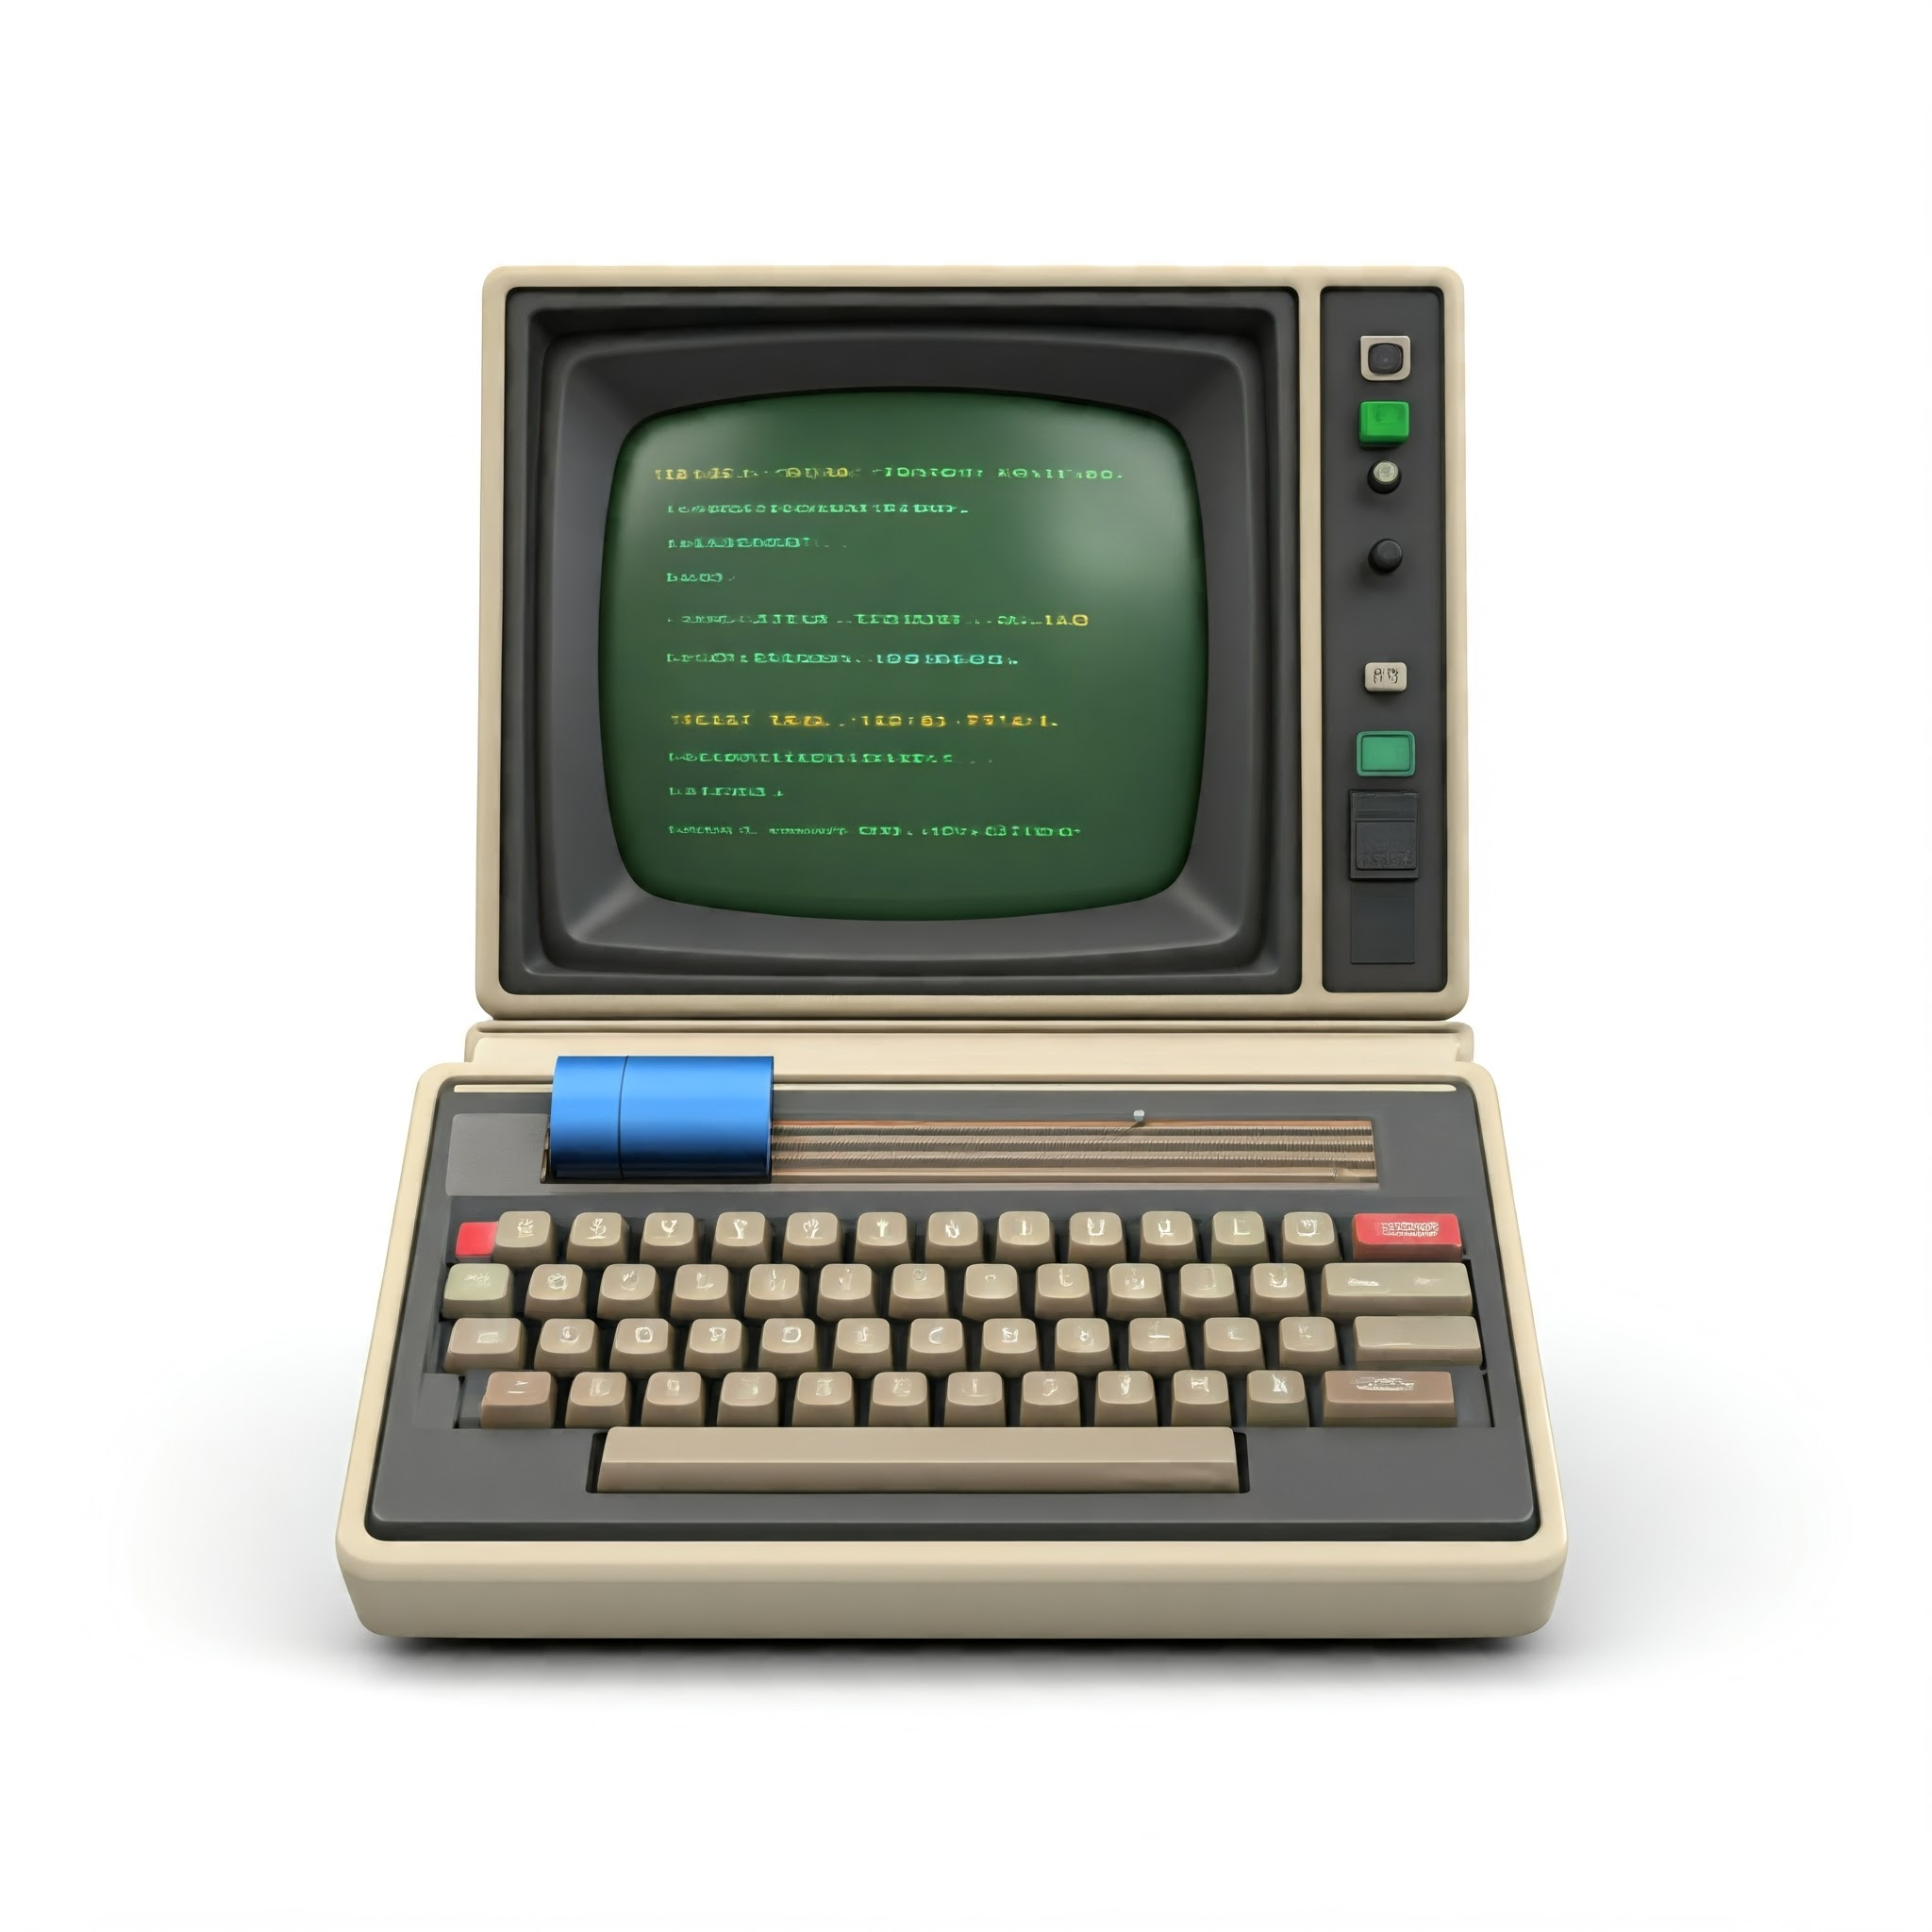
\includegraphics[width=1\textwidth ]{images/copertina2.jpeg}
    }
\end{figure}
\vfill 
\centering 
\includegraphics[width=0.4\textwidth ]{../../preamble/Stemma_sapienza.png} \acc
\centering \Large \color{sapienza}Facoltà di Ingegneria dell'Informazione,
Informatica e Statistica\\
Dipartimento di Informatica
\end{titlepage}

%===================FINE COPERTINA======================%
\newpage
\pagecolor{cartaRiciclata}%\setmainfont{Algerian}
\Large
Questo documento è distribuito sotto la licenza 
\color{blue}\href{https://www.gnu.org/licenses/fdl-1.3.txt}{GNU}\color{black},  
è un resoconto degli appunti (eventualmente integrati con libri di testo) tratti dalle lezioni del corso di Automi, Calcolabilità e Complessità
\hphantom{a}per la laurea 
triennale in Informatica. Se dovessi notare errori, ti prego di segnalarmeli.
\vfill
\begin{figure}[h!]
    \raggedright
    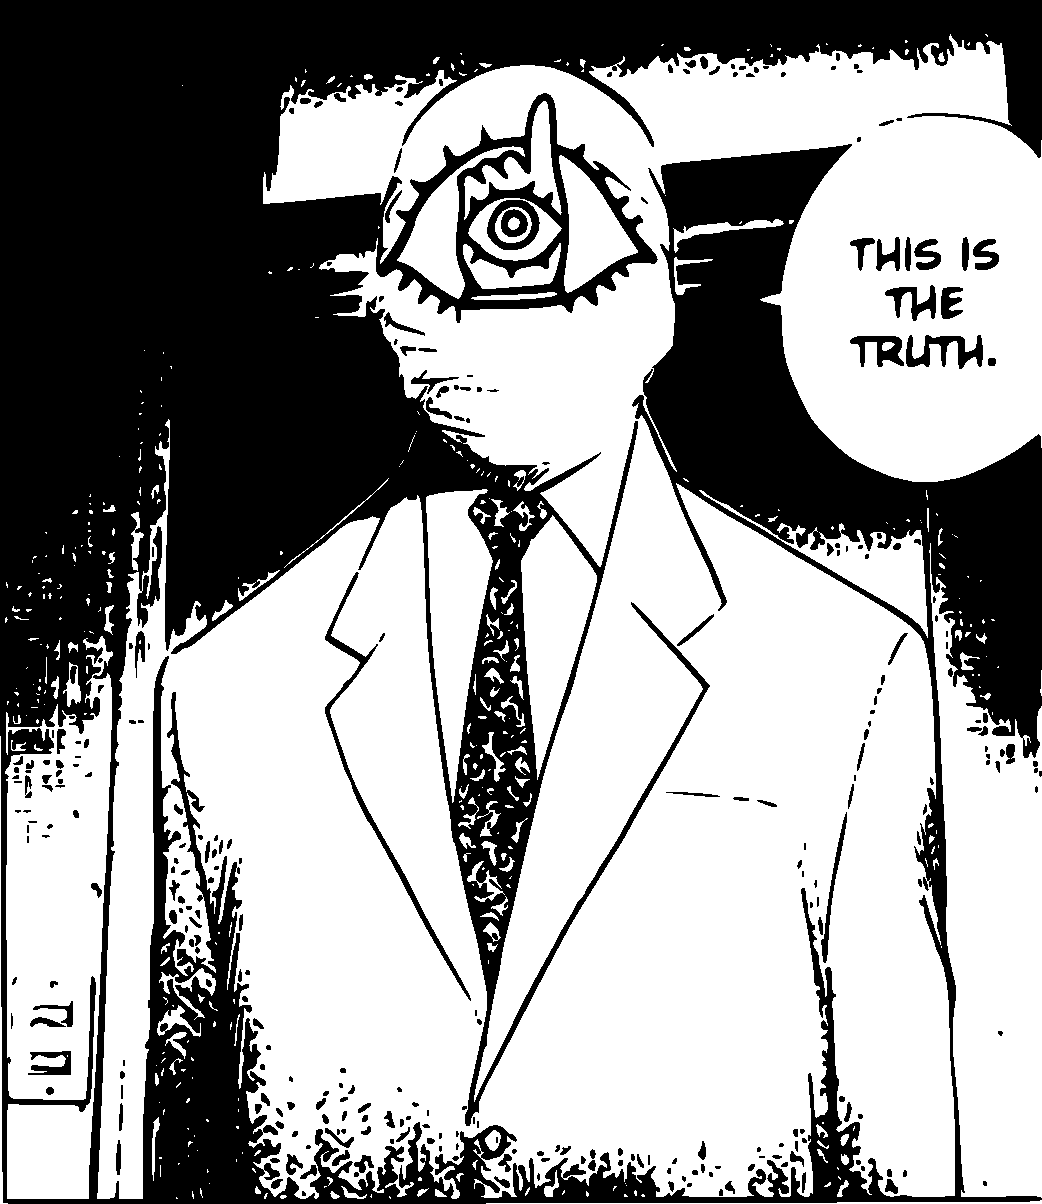
\includegraphics[width=0.4\textwidth,right ]{../../preamble/tomodachi.pdf} 
\end{figure}
\newpage %\setmainfont{Times New Roman}
\normalsize
\tableofcontents 
\newpage

%==================FOOTER e HEADER=======================%
\fancyhf{}
\fancyhead[L]{\nouppercase{\leftmark}}
\fancyhead[R]{Sezione \thesection}
\fancyfoot[C]{\thepage}
\fancyfoot[L]{Appunti di Automi, Calcolabilità e Complessità}
\fancyfoot[R]{ Marco Casu}
%\fancyfoot[R]{\setmainfont{Palace Script MT}\huge Marco Casu \setmainfont{Times New Roman}}
%==================FOOTER e HEADER=======================%

%Ricorda del comando \flowerLine per separare le sottosezioni. Le sezioni si separano nelle diverse pagine

%==================INIZIO======================%
\chapter{Automi}
\section{Linguaggi Regolari}
Un \textit{automa a 
stati finiti} è, seppure limitato nella memoria e nella gestione 
dell'input, il più 
semplice modello di computazione. Un automa può interagire con l'input 
esclusivamente "scorrendolo" in maniera sequenziale.\acc 
\textbf{Esempio} : Si vuole modellare una semplice porta con sensore, che 
si apre quando qualcuno si trova nelle vicinanze.
\begin{center}
    \includegraphics[width=0.6\textwidth ]{images/porta.eps}
\end{center}
Un automa che modella il problema è il seguente :\begin{center}
    
    
    \begin{tikzpicture} [node distance = 6cm, on grid, auto]
        \node (aperta)[state, left] {aperta};
        \node (chiusa)[state, right = of aperta] {chiusa};
        \path [-stealth, thick]
        (aperta) edge [loop left]  node {rileva persone}()
        (chiusa) edge [loop right]  node {nessuno}()
        (aperta) edge [bend left] node {nessuno}   (chiusa)
        (chiusa) edge [bend left] node {rileva persone}   (aperta);
    \end{tikzpicture}
\end{center} 
Un automa ha alcuni stati speciali, come quello iniziale, indicato 
con un apposita freccia, e degli stati detti \textit{di accettazione}, 
ossia stati in cui deve necessariamente terminare la computazione per 
essere definita valida, vengono rappresentati con un doppio cerchio.
\acc 
Il modello di calcolo degli automi è riconducibile al concetto di 
\textit{linguaggio regolare}, che verrà formalizzato in seguito, 
segue ora una definizione formale di automa.\acc 
\defi{(DFA)} : Un DFA (Deterministic Finite Automa) è una 
5-tupla, $(Q,\Sigma,\delta, q_0, F)$ di cui\begin{itemize}
    \item $Q$ è l'insieme degli stati possibili 
    \item $\Sigma$ è l'alfabeto che compone le stringhe in input 
    \item $\delta$ è una mappa $Q\times \Sigma \rightarrow Q$ detta 
    \textit{funzione di transizione}. 
    \item $q_0\in Q$ è lo stato iniziale. 
    \item $F\subseteq Q$ è l'insieme degli stati di accettazione.
\end{itemize}
\begin{figure}[h!]
    \centering
    \begin{tikzpicture} [node distance = 3cm, on grid, auto]

        \node (q0) [state, initial, accepting, initial text = {}] {$q_1$};
        \node (q1) [state, above right = of q0] {$q_2$};
        \node (q2) [state, below right = of q1] {$q_3$};
        
        \path [-stealth, thick]
            (q0) edge node {0,1}   (q1)
            (q1) edge node {1}   (q2)
            (q1) edge [loop above]  node {0}()
            (q2) edge node {1,0} (q0);
        \end{tikzpicture}
        \caption{semplice automa}
        \label{fig:automaSemplice}
\end{figure}
Nell'esempio in figura \ref{fig:automaSemplice}, si ha che\begin{itemize}
    \item $Q=\{q_1,q_2,q_3\}$
    \item $\Sigma = \{0,1\}$
    \item $F=\{q_1\}$
    \item $q_0=q_1$
    \item $\delta =\;\;\; $ \begin{tabular}{c|c|c}
        & 0     & 1     \\ \hline
  $q_1$ & $q_2$ & $q_2$ \\ \hline
  $q_2$ & $q_2$ & $q_3$ \\ \hline
  $q_3$ & $q_1$ & $q_1$
  \end{tabular}
\end{itemize}
Sia $D$ un DFA, chiamiamo \textbf{linguaggio dell'automa}, e denotiamo 
$L(D)$, l'insieme delle stringhe che date in input a $D$ fanno si che 
$D$ termini su uno stato di accettazione.
\begin{figure}[h!]
    \centering
    \begin{tikzpicture} [node distance = 3cm, on grid, auto]
        \node (q0)[state, left, initial] {$q_1$};
        \node (q1)[state, right = of q0, accepting] {$q_2$};
        \path [-stealth, thick]
        (q0) edge [loop above]  node {0}()
        (q1) edge [loop above]  node {1}()
        (q0) edge [bend left] node {1}   (q1)
        (q1) edge [bend left] node {0}   (q0);
        \end{tikzpicture}
        \caption{il linguaggio di tale automa 
        risulta essere composto dalle stringhe che 
        terminano con $1$}
        \label{fig:automaSemplice2}
\end{figure}
Per definire formalmente un linguaggio di un automa, è 
necessario introdurre la \textbf{funzione di transizione estesa}:
$$ \delta^*(q,\epsilon)=\delta(q,\epsilon)$$
$$\delta^*(q,ax)=\delta^*(\delta(q,a),x)$$
dove
$$ a\in \Sigma,\;\;x\in \Sigma^*,\;\;\epsilon = \text{ stringa vuota}$$
$\Sigma^*$ è l'insieme di tutte le stringhe formate dall'alfabeto 
$\Sigma$. Passiamo ora alla definizione di \textbf{configurazione}, essa 
rappresenta lo stato dell'automa ad un certo punto della 
computazione, essa è formata da una coppia 
$$ Q\times \Sigma^*$$
Rappresentante uno stato, ed una stringa di input rimanente da 
computare.\acc 
Un \textbf{passo della computazione} in un automa rappresenta 
una transizione da una configurazione ad un altra, è una 
relazione binaria $\vdash_D : Q\times \Sigma^*$ tale che 
$$ 
(p,ax)\vdash_D (q,x)\iff \delta(p,a)=q \;\;\text{ dove }\;\;
p,q\in Q,\;\;a\in\Sigma,\;\;x\in\Sigma^*$$
Si può estendere la definizione di passo di computazione, 
considerando la sua \textit{chiusura transitiva} 
$\vdash_D^*$. Essa si ottiene aggiungendo a $\vdash_D$ tutte 
le coppie in $ Q\times \Sigma^*$ che rendono 
la relazione chiusa rispetto la riflessività e rispetto 
la transitività.
$$ \begin{matrix}
    (q,aby)\vdash_D (p,by) \;\land\;  
    (p,by)\vdash_D (ry) \implies 
    (q,aby)\vdash_D^*(r,y)
\end{matrix}$$
Ad esempio, nell'automa in figura \ref{fig:automaSemplice2}, 
risulta chiaro che 
$$\begin{cases}
    (q_1,011)\vdash_D (q_1,11)\\
    (q_1,11) \vdash_D (q_2,1)\\
    (q_2,1) \vdash_D (q_2,\epsilon)
\end{cases} \implies
(q_1,011) \vdash_D^* (q_2,\epsilon)$$
Inoltre$$ \begin{matrix}
    \delta^*(q_1,011) = \\ 
    \delta^*(q_1,11)  = \\ 
    \delta^*(q_2,1) = \\ 
    \delta^*(q_2,\epsilon) = q_2
\end{matrix}$$
Se non specificato diversamente, con $\epsilon$ verrà indicata 
la stringa vuota. Utilizzando le precedenti definizioni, è possibile definire formalmente 
quali sono gli input accettati da un DFA.\acc 
\defi{} : Sia $D=(Q,\Sigma,\delta, q_0, F)$ un DFA, e sia $x\in \Sigma^*$ una stringa, essa 
è \textbf{accettata} da $D$ se $$ \delta^*(q_0,x)\in F$$
Il \textbf{linguaggio riconosciuto} da $D$ è \eqImportante{$ L(D)=\{x\in \Sigma^*|\delta^*(q_0,x)\in F\}$}
\defi{(Linguaggi Regolari)} : L'insieme dei linguaggi regolari, denotato $REG$, contiene tutti 
i linguaggi, tali che esiste un DFA che li ha come linguaggi riconosciuti.
\eqImportante{$ REG = \{L\;\;|\;\;\exists D=(Q,\Sigma,\delta, q_0, F) \text{ t.c. } L\in \Sigma^* \land L(D)=L\}$}
Uno fra gli scopi di questo corso riguarda il capire come progettare automi, e capire se, 
ogni linguaggio è regolare, o ce ne sono alcuni che non possono essere riconosciuti da 
alcun possibile DFA. 
\subsection{Esempi di DFA}
Vediamo in questa sezione alcuni semplici esempi di DFA.\acc 
\textbf{Esempio 1)} Si vuole progettare un DFA che accetti il seguente linguaggio 
$$ \{x\in\{0,1\}^* \;|\;w_h(x)\ge 3 \}$$
Si ricordi come 
$$ w_h(x) = \text{ occorrenze di 1 in }x$$
\begin{figure}[h!]
    \centering
    \begin{tikzpicture} [node distance = 2cm, on grid, auto]
        \node (q0)[state, left, initial] {$q_0$};
        \node (q1)[state, right = of q0] {$q_1$};
        \node (q2)[state, right = of q1] {$q_2$};
        \node (q3)[state, right = of q2, accepting] {$q_3$};
        \path [-stealth, thick]
        (q0) edge [loop above]  node {0}()
        (q1) edge [loop above]  node {0}()
        (q2) edge [loop above]  node {0}()
        (q3) edge [loop right]  node {1,0}()
        (q0) edge [bend left] node {1}   (q1)
        (q1) edge [bend left] node {1}   (q2)
        (q2) edge [bend left] node {1}   (q3);
        \end{tikzpicture}
        \caption{Esempio (1) di DFA}
        \label{fig:DFAExample1}
\end{figure}
Una volta progettato il DFA, è anche importante dimostrarne la correttezza, ossia dare una prova 
matematico che l'automa in questione accetti il linguaggio.\begin{itemize}
    \item Se $x\in L(D)$ allora $D$ accetta $x$
    \item Se $D$ accetta $x$ allora $w_h(x)\ge 3$
\end{itemize}
In questo, e nei seguenti casi, essendo i DFA estremamente semplici, risulta ovvio che 
accettino il dato linguaggio, in casi più avanzati, sarà necessario fornire una dimostrazione 
rigorosa.\acc 
\textbf{Esempio 2)} Si vuole progettare un DFA che accetti il seguente linguaggio 
$$ \{x\in\{0,1\}^* \;|\;x=1y \land y \in  \{0,1\}^*\}$$
Appunto sulla notazione : Se $a\in \Sigma^*$ e $b\in \Sigma^*$, allora con $ab$ si 
denota la concatenazione di stringhe.\acc
\begin{figure}[h!]
    \centering
    \begin{tikzpicture} [node distance = 2cm, on grid, auto]
        \node (q0)[state, left, initial] {$q_0$};
        \node (q1)[state, below = of q0] {$q_1$};
        \node (q2)[state, right = of q0, accepting] {$q_2$};
        \path [-stealth, thick]
        (q1) edge [loop left]  node {0,1}()
        (q2) edge [loop above]  node {0,1}()
        (q0) edge [bend left] node {0}   (q1)
        (q0) edge [bend left] node {1}   (q2);
        \end{tikzpicture}
        \caption{Esempio (2) di DFA}
        \label{fig:DFAExample2}
\end{figure}\acc 
Nell'esempio (2), quando dallo stato $q_0$ il DFA riceve in input $0$, la computazione cade su uno stato 
"buco nero", dalla quale non si può uscire a prescindere dall'input, l'operazione che fa 
cadere in questo stato è da considerarsi "non definita" in quanto non porterà mai la computazione 
a terminare su uno stato accettabile, è quindi comodo rimuovere tale stato dal diagramma.
\begin{figure}[h!]
    \centering
    \begin{tikzpicture} [node distance = 3cm, on grid, auto]
        \node (q0)[state, left, initial] {$q_0$};
        \node (q2)[state, right = of q0, accepting] {$q_2$};
        \path [-stealth, thick]
        (q2) edge [loop above]  node {0,1}()
        (q0) edge [bend left] node {1}   (q2);
        \end{tikzpicture}
        \caption{Esempio (2.1) di DFA}
        \label{fig:DFAExample2.1}
\end{figure}\acc 
Anche in questo caso la dimostrazione della correttezza risulta banale.\acc 
\textbf{Esempio 3)} Si vuole progettare un DFA che accetti il seguente linguaggio 
$$ \{x\in\{0,1\}^* \;|\;x=0^n1,\;\;n\in \N\}$$
Con $0^n1$ si intende una stringa che sia composta esclusivamente da $0$, ma con un $1$ come 
ultimo termine, ad esempio : $$0000000000000001$$\newpage
\begin{figure}[h!]
    \centering
    \begin{tikzpicture} [node distance = 3cm, on grid, auto]
        \node (q0)[state, left, initial] {$q_0$};
        \node (q1)[state, right = of q0] {$q_1$};
        \node (q2)[state, right = of q1, accepting] {$q_2$};
        \path [-stealth, thick]
        (q1) edge [loop above]  node {0}()
        (q0) edge  node {0}   (q1)
        (q1) edge  node {1}   (q2);
        \end{tikzpicture}
        \caption{Esempio (3) di DFA}
        \label{fig:DFAExampl3}
\end{figure}
\flowerLine 
\section{Operazioni sui Linguaggi}
Lo studio delle proprietà dei linguaggi regolari può fornire opportune accortezze
utili nella progettazione di automi, siccome i linguaggi sono insiemi di stringhe costruiti 
su un alfabeto $\Sigma$, essi godono delle operazioni insiemistiche.\acc
Risulta utile definire formalmente la concatenazione fra stringhe, siano 
$$ x = a_1,a_2\dots,a_n\;\;\;\;\;\;\;\;\;\;\;\;y = b_1,b_2\dots,b_n $$
due stringhe, esse possono essere concatenate 
$$xy=  a_1,a_2\dots,a_n,b_1,b_2\dots,b_n $$
L'operazione di concatenazione non è commutativa, può essere definita ricorsivamente in tal 
modo : 
$$ x(ya) = (xy)a$$ 
dove 
$$x,y\in \Sigma^*\;\;\;\;\;\;\;\;\;a\in \Sigma$$
Siano $L_1,L_2$ due 
linguaggi regolari in $REG$ (per semplicità, definiti su uno stesso alfabeto $\Sigma$), e 
sia $n$ un numero naturale, sono 
definite su di essi le seguenti operazioni : \begin{itemize}
    \item \textbf{unione} : $L_1\cup L_2 = \{x\in\Sigma^*\;|\;x\in L_1\lor x\in L_2\}$
    \item \textbf{intersezione} : $L_1\cap L_2 = \{x\in\Sigma^*\;|\;x\in L_1\land x\in L_2\}$
    \item \textbf{complemento} : $\lnot L_1=\{x\in\Sigma^*\;|\;x\notin L_1\}$
    \item \textbf{concatenazione} : $L_1 \circ L_2 = \{xy\;|\;x\in L_1\land y\in L_2\}$
    \item \textbf{potenza} : $L_1^n = \smash{\underbrace{L_1\circ L_1\circ L_1,\dots\circ L_1}_{n\ \text{volte}}}\vphantom{1}$\acc
    \item \textbf{star} : $L_1^* = \{x_1,x_2\dots,x_k\;|\; k\in \Z^+ \land x_i \in L_1\}$ \\ 
    Si può definire anche diversamente $$L_1^* = \bigcup_{k=0}^\infty L_1^k $$
\end{itemize}
\textit{Esempio di concatenazione e potenza} : 
$$\Sigma= \{a,b\}\;\;\;\; L_1 = \{a,ab,ba\}\;\;\;\; L_2 = \{ab,b\}\;\;\;\; L = \{a,ab,ba\}$$
$$L_1\circ L_2 = \{aab,ab,abab,abb,baab,bab\} $$
$$ L^2=\{aa,aab,aba,abab,abba,baa,baba\}$$
\teo{(Chiusura di $REG$)} La classe dei linguaggi regolari $REG$, è chiusa rispetto a tutte le 
operazioni appena elencate, siano $L_1$ ed $L_2$ due linguaggi regolari, allora :
$$\begin{matrix}
    L_1\cup L_2 \in REG && L_1\circ L_2 \in REG &&
    L_1\cap L_2 \in REG \\ \\ L_1^n \in REG &&
    \lnot L_1 \in REG && L_1^* \in REG
\end{matrix}$$
\dimo{(unione ed intersezione)} Siano $L_1$ ed $L_2$ due linguaggi regolari, considero due DFA, per semplicità, con lo stesso alfabeto
$$ 
D_1 = (Q_1,\Sigma,\delta,q_1,F_1)
$$
$$ 
D_2 = (Q_2,\Sigma,\delta,q_2,F_2)
$$
tali che 
$$ L(D_1)=L_1 \ \land \ L(D_2)=L_2$$
Si costruisce un DFA che simula contemporaneamente l'esecuzione di $D_1$ e $D_2$, in cui gli stati possibili saranno 
le possibili combinazioni di coppie di stati. Si definisce $D=(Q,\Sigma,\delta,q_0,F)$ tale che 
\begin{itemize}
    \item $Q=Q_1\times Q_2=\{(r_1,r_2) \|\ r_1\in Q_1 \land r_2\in Q_2\}$
    \item $\delta((r_1,r_2),a)=(\delta(r_1,a),\delta(r_2,a))$ dove $a\in\Sigma$ e $(r_1,r_2)\in Q$
    \item $q_0=(q_1,q_2)$
    \item $F=(F_1\times Q_2)\cup (Q_1\times F_2)=\{(r_1,r_2)\|\ r_1\in F_1\lor r_2\in F_2\}$
\end{itemize}
Nel caso si dovesse dimostrare la proprietà dell'intersezione, si avrebbe che \begin{itemize}
    \item $F=F_1\times F_2$
\end{itemize}
A questo punto risulta chiaro che 
\begin{enumerate}[(i)] 
    \item $x\in L_1\cup L_2\implies x\in L(D)$
    \item $x\in L(D)\implies x\in L_1\cup L_2\;\;\blacksquare$ 
\end{enumerate}
\dimo{(complemento)} : Sia $L$ un linguaggio regolare, e $D$ un automa che lo accetta $L(D)=L$. Si vuole dimostrare 
che esiste un automa che accetti $L^C = \{w\in \Sigma^* \ |\ w\notin L\}$. Essendo 
$$ D=(Q,\Sigma,\delta,q_0,F)$$
considero 
$$ D'=(Q,\Sigma,\delta,q_0,F^C)$$
dove  $F^C=Q\backslash F$. Supponiamo che $w\in L^C$, allora sicuramente, se data come input a $D'$, 
la computazione terminerà in uno stato che non è in $F$, dato che, per definizione, se terminasse in $F$, sarebbe 
accettato da $D$, ma $L^C$ contiene tutte le stringhe che non sono accettate da $D$, quindi\begin{itemize}
    \item $w\in L^C$
    \item  la computazione termina in uno stato $q\in F^C$ 
    \item $D'$ accetta $w$ 
    \item $L^C$ è un linguaggio regolare. $\blacksquare$ 
\end{itemize} 
Per dimostrare la proprietà di concatenazione, è necessario introdurre un nuovo concetto. 
\flowerLine 
\section{Non Determinismo}
Si può generalizzare il modello di DFA, in modo tale che la lettura di un input non scaturisca il passaggio da 
uno stato ad un'altro, ma da uno stato ad un insieme di stati, tale generalizzazione è 
detta \textit{Non-Deterministic Finite Automa}.\acc 
\defi{(NFA)} : Un NFA è una tupla $N=(Q,\Sigma,\delta,q_0,F)$ tale che \begin{itemize}
    \item $Q,\Sigma,q_0,F$ condividono la definizione con i loro corrispettivi nel DFA 
    \item $\delta : Q\times \Sigma_\epsilon\rightarrow\mathcal{P}(Q)$ \begin{itemize}
        \item $\Sigma_\epsilon = \Sigma \cup \{\epsilon\}$
        \item $\mathcal{P}(Q)$ è l'insieme delle parti di $Q$
    \end{itemize}
\end{itemize}
Una computazione in un NFA è paragonabile ad una computazione parallela, in cui un 
input può risultare in diversi \textit{rami} di computazione. Una funzione di transizione di un 
$NFA$ inoltre accetta la stringa vuota $\epsilon$, se la computazione finisce in uno stato in cui è 
presente un arco di questo tipo, verrà considerata anche una diramazione verso quell'arco a prescindere 
dall'input. \acc 
Una computazione si può rappresentare graficamente con un albero, se una delle diramazioni possibili termina in 
uno stato accettabile, allora la stringa in input è accettata. 
\begin{figure}[h!]
    \centering
    \begin{tikzpicture} [node distance = 2cm, on grid, auto]
        \node (q0)[state, left, initial] {$q_1$};
        \node (q1)[state, right = of q0] {$q_2$};
        \node (q2)[state, right = of q1] {$q_3$};
        \node (q3)[state, right = of q2, accepting] {$q_4$};
        \path [-stealth, thick]
        (q0) edge [loop above]  node {0,1}()
        (q0) edge [bend left] node {1}   (q1)
        (q1) edge [bend left] node {0,1}   (q2)
        (q2) edge [bend left] node {0,1}   (q3);
    \end{tikzpicture}
    \caption{Esempio di NFA}
    \label{fig:NFAExample1}
\end{figure}\acc
Sia $N$ l'NFA mostrato in figura \ref{fig:NFAExample1}, si ha 
$$ L(N)=\{x\in\{0,1\}^*\|\ x\text{ ha $1$ come terzultimo valore }\}$$
Si può visualizzare il seguente albero di computazione data come input una stringa $w$ :
$$w=10110$$\begin{center}
    \includegraphics[width=0.7\textwidth ]{images/alberoCalc.eps}
\end{center}
Essendo che la traccia di sinistra accetta $w$, allora $N$ accetta $w$.\acc 
È necessario estendere il concetto di \textit{configurazione} per gli NFA, essa, rappresentante 
uno stato della computazione, sarà una coppia 
$$ (q,x)\in Q\times \Sigma_\epsilon$$
E diremo che 
$$ (p,ax)\vdash_N (q,x)\iff q\in \delta(p,a)$$
dove 
$$p,q\in Q \ \ \ \ a\in \Sigma_\epsilon\ \ \ \ x\in \Sigma_\epsilon^*$$
Si considera ora la chiusura transitiva di $\vdash_N$, denotata $\vdash_N^*$, se $w$ è una stringa ed 
$N$ un NFA, si ha che 
$$ w\in L(N)\iff \exists q\in F \|\ (q_0,w)\vdash_N^* (q,\epsilon)$$
Consideriamo adesso l'unione di due NFA, risulta particolarmente semplice da definire, siano $N_1$ e $N_2$ due 
NFA, che per semplicità, condividono l'alfabeto 
$$ 
N_1=\{Q_1,\Sigma_\epsilon,\delta_1,q_1,F_1\}
$$$$ 
N_2=\{Q_2,\Sigma_\epsilon,\delta_2,q_2,F_2\}
$$
Definisco un nuovo NFA $N=(Q,\Sigma_\epsilon,\delta,q_0,F)$ tale che \begin{itemize}
    \item $Q=Q_1\cup Q_2$
    \item $F=F_1\cup F_2$
    \item Siano $q\in Q$ e $a\in\Sigma_\epsilon$ : 
    $$ 
        \delta(q,a)=\begin{cases}
            \delta_1(q,a) \text{ se }q\in Q_1\\
            \delta_2(q,a) \text{ se }q\in Q_2\\
            \{q_1,q_2\} \text{ se }q=q_0  \ \land\ a=\epsilon \\
            \emptyset \text{ se }q=q_0\ \land \ a\ne \epsilon 
        \end{cases}
    $$
\end{itemize}
Si avrà che $L(N)=L(N_1)\cup L(N_2)$\begin{center}
    \begin{figure}[h!]
        \centering 
        \includegraphics[width=0.6\textwidth ]{images/UnioneNFA.eps}
        \caption{Unione di due NFA}
        \label{fig:NFAUnion}
    \end{figure}
\end{center}
Denotiamo $\mathcal{L}(DFA)$ l'insieme dei linguaggi accettati da un qualsiasi DFA, che per definizione è $REG$, e denotiamo, in maniera analoga 
$\mathcal{L}(NFA)$. \acc 
\teo{} : L'insieme dei linguaggi accettati da un qualsiasi DFA, e quello dei linguaggi accettati 
da un qualsiasi NFA coincidono $$\mathcal{L}(DFA)=\mathcal{L}(NFA)=REG$$
\dimo{} Il caso $\mathcal{L}(DFA)\subseteq\mathcal{L}(NFA)$ è banale e non verrà dimostrato. Si vuole dimostrare che 
se $L$ è accettato da un generico NFA, allora esiste un DFA che accetta $L$, l'idea è quella di "simulare" un NFA 
tramite un DFA che rappresenti ogni possibile stato di computazione.



Sia $N=(Q_N,\Sigma,\delta_N,q_{0_N},F_N)$ un NFA, e sia $L=L(N)$. Si considera un DFA 
$D=(Q_D,\Sigma,\delta_D,q_{0_D},F_D)$ tale che \begin{itemize}
    \item $Q_D=\mathcal{P}(Q_N)$
    \item $q_{0_D}=\{q_{0_N}\}$
    \item $F_D=\{R\in Q_D | R\cap F_N\ne \emptyset\}$, ovvero, $D$ accetta tutti gli insiemi in cui compare almeno 
    un elemento accettato da $N$.
    \item Sia $R\in Q_D$ e $a\in\Sigma$, si definisce $\displaystyle\delta_D(R,a)=\bigcup_{r\in R}\delta_N(r,a)$
\end{itemize}
Questo caso non tiene conto di un NFA in cui sono presenti degli $\epsilon$-archi. Supponiamo che vi siano,  sia 
$R\in Q_D$, si definisce la funzione estesa $E$ definita come segue 
$$ E(R)=\{q\in Q_N \|\ q\text{ può essere raggiunto da un qualsiasi stato  }r\in R\text{ attraverso zero o 
più }\epsilon\text{-archi }\}$$
Cambia la definizione del DFA utilizzato per la dimostrazione \begin{itemize}
    \item $q_{0_D}=E(\{q_{0_N})\}$
    \item $\displaystyle\delta_D(R,a)=\bigcup_{r\in R}E(\delta_N(r,a))$
\end{itemize}
È chiaro che $D$ tiene traccia di tutte le possibili computazioni di $N$, ed accetta $L$, ossia $L(D)=L(N)$. $\blacksquare$\acc 
\textbf{Esempio} : Si consideri l'NFA $N$ definito come segue
\begin{figure}[h!]
    \centering
    \begin{tikzpicture} [node distance = 2cm, on grid, auto]
        \node (q0)[state,accepting, left, initial] {$q_1$};
        \node (q1)[state, below = of q0] {$q_2$};
        \node (q2)[state, right = of q1] {$q_3$};
        \path [-stealth, thick]
        (q1) edge [loop left]  node {$a$}()
        (q0) edge [bend right] node {$b$}   (q1)
        (q0) edge [bend right] node {$\epsilon$}   (q2)
        (q2) edge [bend right] node {$a$}   (q0)
        (q1) edge [bend right] node {$a,b$}   (q2);
    \end{tikzpicture}
    \caption{$N=(Q_N,\Sigma,\delta_N,q_{0_N},F_N)$}
    \label{fig:NFAExample2}
\end{figure}\acc
Si costruisce un DFA $D=(Q_D,\Sigma,\delta_D,q_{0_D},F_D)$ con le seguenti specifiche (per comodità, l'elemento $\{q_i,q_j\dots,q_k\}$ verrà 
denotato $p_{ij\dots k}$), mostrato in figura \ref{fig:DFAgenerated}
\begin{figure}[h!]
    \centering
    \begin{tikzpicture} [node distance = 3.5cm, on grid, auto]
        \node (p13)[state,accepting, initial above] {$p_{13}$};
        \node (p3)[state,left = of p13] {$p_{3}$};
        \node (p0)[state,above = of p3] {$p_{0}$};
        \node (p1)[state,above = of p13,accepting] {$p_{1}$};
        \node (p2)[state,right = of p1] {$p_{2}$};
        \node (p23)[state,right = of p13] {$p_{23}$};
        \node (p12)[state,right = of p2,accepting] {$p_{12}$};
        \node (p123)[state,right = of p23,accepting] {$p_{123}$};
        \path [-stealth, thick]
        (p0) edge [loop left]  node {$a,b$}()
        (p13) edge [loop left]  node {$a$}()
        (p123) edge [loop right]  node {$a$}()
        (p1) edge [bend left] node {$b$}   (p2)
        (p13) edge  node {$b$}   (p2)
        (p2) edge  node {$b$}   (p3)
        (p2) edge  node {$a$}   (p23)
        (p123) edge [bend left] node {$b$}   (p23)
        (p12) edge  node {$a,b$}   (p23)
        (p23) edge [bend left, below] node {$b$}   (p3)
        (p23) edge  node {$a$}   (p123)
        (p3) edge [bend left] node {$b$}   (p0)
        (p3) edge [bend right] node {$a$}   (p13)
        (p1) edge [bend right] node {$a$}   (p0);
    \end{tikzpicture}
    \caption{grafico di $D$}
    \label{fig:DFAgenerated}
\end{figure}
\begin{itemize}
    \item $Q_D=\{p_0,p_1,p_2,p_3,p_{12},p_{13},p_{23},p_{123}\}$
    \item $E(q_{0_N})=\{q_1,q_3\}\implies q_{0_D}=p_{13}$
    \item $F_D=\{p_1,p_{12},p_{13},p_{123}\}$
    \item la funzione $\delta_D$ si definisce osservando il grafico di $N$\begin{itemize}
        \item $\delta_N(q_2,a)=\{q_2,q_3\}\implies \delta_D(p_2,a)=p_{23}$
        \item $\delta_N(q_2,b)=\{q_3\}\implies \delta_D(p_2,a)=p_{3}$
        \item $\delta_N(q_1,a)=\emptyset\implies \delta_D(p_1,a)=p_0$
        \item $\delta_N(q_1,b)=\{q_2\}\implies \delta_D(p_1,b)=p_{2}$
        \item etc...
    \end{itemize}
\end{itemize}

L'introduzione degli automi non deterministici è stata necessaria in principio per la dimostrazione della chiusura 
di $REG$ rispetto le operazioni di concatenazione e star.\acc 
\teo{} $REG$ è chiusa per concatenazione.\acc 
\dimo{} Siano $L_1$ ed $L_2$ due linguaggi regolari, esistono quindi due NFA 
$$ N_1=(Q_1,\Sigma_\epsilon,\delta_1,q_0^1,F_1)\ \ \ \ \ \  
N_2=(Q_2,\Sigma_\epsilon,\delta_2,q_0^2,F_2)$$
tali che $L(N_1)=L_1 \ \land \ L(N_2)=L_2$. Si costruisce un NFA $N=(Q,\Sigma_\epsilon,\delta,q_0,F)$, l'idea è quella 
di concatenare le ramificazioni di $N_1$ ad $N_2$.
\begin{center}
    \begin{figure}[h!]
        \centering 
        \includegraphics[width=1\textwidth ]{images/concatenazioneChiusa.eps}
        \caption{schema di $N$}
        \label{fig:concatenazioneChiusa}
    \end{figure}
\end{center}
Un NFA di questo tipo computerà una stringa in $L_1$, se finirà in uno stato di $F_1$, andrà nello stato iniziale 
di $N_2$, è chiaro che l'automa accetta solamente una concatenazione di stringhe fra $L_1$ ed $L_2$. \begin{itemize}
    \item $Q=Q_1\cup Q_2$
    \item $q_0=q_0^1$
    \item $F=F_2$
    \item per $a\in\Sigma_\epsilon$ e $q\in Q$ si ha $\delta(q,a)=\begin{cases}
        \delta_1(q,a) \text{ se }q\in Q_1\land q\notin F_1\\ 
        \delta_1(q,a)\text{ se }q\in F_1\land a\ne \epsilon\\ 
        \delta_1(q,a)\cup\{q_0^2\}\text{ se }q\in F_1\land a= \epsilon\\ 
        \delta_2(q,a)\text{ se }q\in Q_2\\
    \end{cases}$
\end{itemize}
Si ha quindi che $L(N)=L_1\circ L_2$. $\blacksquare$\acc 
\teo{} $REG$ è chiusa per star.\acc 
\dimo{} Sia $L\in REG$ e sia $N=(Q,\Sigma_\epsilon,\delta,q_{0},F)$ un NFA tale che $L(N)=L$. Considero un NFA $N^*=(Q^*,\Sigma_\epsilon,\delta^*,q_{0}^*,F^*)$,
 identico ad $N$, con opportune 
modifiche, lo stato $q_0$ iniziale di $N$ non è iniziale in $N^*$, 
ed ogni stato finale ha una $\epsilon$-arco verso $q_0$.\begin{itemize}
    \item $Q^*=Q\cup\{q_0^*\}$
    \item $q_0^*$ è un nuovo stato 
    \item $F^*=F\cup\{q_0^*\}$ questo perché in $L^*$ è presente la stringa vuota
    \item per $a\in\Sigma_\epsilon$ e $q\in Q^*$ si ha $\delta^*(q,a)=\begin{cases}
        \delta(q,a) \text{ se }q\in Q\land q\notin F\\ 
        \delta(q,a) \text{ se }q\in F\land a\ne \epsilon\\
        \delta(q,a)\cup\{q_0\} \text{ se }q\in F\land a= \epsilon\\
        \{q_0\}\text{ se }q=q_0^*\land a =\epsilon\\ 
        \emptyset \text{ se }q=q_0^*\land a\ne \epsilon
    \end{cases}$
\end{itemize}
\begin{center}
    \begin{figure}[h!]
        \centering 
        \includegraphics[width=1\textwidth ]{images/starChiusa.eps}
        \caption{schema di $N^*$}
        \label{fig:starChiusa}
    \end{figure}
\end{center}
\flowerLine 
\section{Espressioni Regolari}
 Un espressione regolare è simile ad un espressione algebrica ma opera sulle stringhe, dato un alfabeto, un'espressione 
 su tale alfabeto rappresenta un insieme di stringhe, un esempio è 
 $$(0|1)0^*$$ 
 Dove $(0|1)\equiv \{0\}\cup \{1\}=\{0,1\}$ e $0^*\equiv\{0\}^*$ quindi $(0|1)0^*\equiv \{0,1\}\circ \{0\}^*$.\acc 
 \defi{(espressione regolare)} : Sia $\Sigma$ un alfabeto, un espressione regolare $r$ su $\Sigma$, denotata 
 $r\in re(\Sigma)$, è definita per induzione \\ 
 \textbf{Caso base}\begin{itemize}
    \item $r=\emptyset\in re(\Sigma)$
    \item $r=\epsilon\in re(\Sigma)$
    \item $r=a\in re(\Sigma)$
 \end{itemize}
 \textbf{Caso induttivo}\begin{itemize}
    \item $r=r_1\cup r_2$ dove $r_1,r_2\in re(\Sigma)$
    \item $r=r_1\circ r_2$ dove $r_1,r_2\in re(\Sigma)$
    \item $r=r_1^*$ dove $r_1\in re(\Sigma)$
 \end{itemize}
L'insieme delle stringhe definite da  $r\in re(\Sigma)$ è il \textit{linguaggio} di $r$ ed è denotato $L(r)$.\acc 
\textbf{Esempio : } Sia $\Sigma = \{0,1\}$\begin{itemize}
    \item $0^*10^*=\{w\ | \ w \text{ ha esattamente un }1\}$
    \item $\Sigma^*1\Sigma^*=\{w\ | \ w \text{ ha almeno un }1\}$
    \item $\Sigma^*001\Sigma^*=\{w\ | \ w \text{ ha la sottostringa }001\}$
\end{itemize}
Per convenzione si definisce $$1^*\emptyset = \emptyset \ \ \ \ \ \ \emptyset^*=\epsilon $$
\teo{ Fondamentale} Sia $\mathcal{L}(DFA)=REG$ l'insieme dei linguaggi accettati da un qualsiasi DFA, e sia 
$\mathcal{L}(re)$   l'insieme dei linguaggi accettati da una qualsiasi espressione regolare, è vero che 
$$\mathcal{L}(re)=\mathcal{L}(DFA)=REG $$
\dimo{} è necessario dimostrare due direzioni\acc
\boxedMath{$\mathcal{L}(re)\subseteq\mathcal{L}(DFA)$} Sia $r$ un espressione regolare, si considera un DFA 
$D_r$ definito come segue, a seconda dei casi\acc 
\textbf{Caso base }\begin{itemize}
    \item $r=\emptyset\implies D_r$ non accetta alcuna stringa 
    \item $r=\epsilon\implies D_r$  accetta la stringa vuota
    \item $r=a\implies D_r$  accetta la $a\in\Sigma$
\end{itemize}
\textbf{Caso induttivo}\begin{itemize}
    \item $r=r_1\cup r_2$, esistono due automi $D_{r_1}$ e  $D_{r_2}$ che accettano rispettivamente $L(r_1)$ 
    e $L(r_2)$, ma allora esiste necessariamente un automa $D_r$ che accetta $L(r_1)\cup L(r_2)$.
    \item $r=r_1\circ r_2$,  esistono due automi $D_{r_1}$ e  $D_{r_2}$ che accettano rispettivamente $L(r_1)$ 
    e $L(r_2)$, ma allora esiste necessariamente un automa $D_r$ che accetta $L(r_1)\circ L(r_2)$.
    \item $r=r_1^*$, esiste un automa $D_{r_1}$  che accetta
     $L(r_1^*)$, ma allora esiste necessariamente un automa $D_r$ che accetta $L(r_1)$.
\end{itemize}
Tali tesi sono vere dato che la classe dei linguaggi regolari è chiusa per le operazioni di star, concatenazione 
ed unione. $\square $\acc 
\boxedMath{$\mathcal{L}(DFA)\subseteq\mathcal{L}(re)$} Sia $L$ un linguaggio regolare, e sia $N$ l'NFA tale che 
$L(N)=L$. Si costruisce un nuovo tipo di NFA che sarà equivalente ad $N$. Tale automa è detto \textit{GNFA}, 
dove la G sta per "Generalizzato", tale automa ha una \textit{forma canonica}, ossia, rispetta le seguenti 
proprietà \begin{itemize}
    \item Lo stato iniziale, ha solo archi uscenti 
    \item Vi è un singolo stato finale, ed ha solo archi entranti
    \item Per ogni coppia di stati (non necessariamente distinti), c'è esattamente un arco.
    \item Ogni arco è etichettato da un espressione regolare.
\end{itemize}
\begin{center}
    \begin{figure}[h!]
        \centering 
        \includegraphics[width=0.4\textwidth ]{images/GNFA.eps}
        \caption{forma di un GNFA}
        \label{fig:GNFA}
    \end{figure}
\end{center}
Più precisamente, sia $G$ un GNFA definito $G=(Q,\Sigma,\delta,q_{start},q_{acc})$ dove 
$$ \delta : Q\backslash \{q_{acc}\} \times Q\backslash \{q_{start}\}\rightarrow re(\Sigma)$$
Dato un generico NFA, è possibile trasformarlo in un GNFA aggiungendo al più due stati (iniziale e 
finale), ed utilizzando gli $\epsilon$-archi per riempire le coppie di stati che non sono collegate.\acc 
La funzione $Convert : GNFA \rightarrow GNFA$ modifica un GNFA restituendone uno equivalente, ma con uno stato in meno. 
Tale funzione è definita in tal modo, sia $k$ il numero di archi di $G$, si esegue $Convert(G)$ \begin{itemize}
    \item Se $k=2$, allora esiste un solo arco fra questi etichettato con un espressione regolare $r$, la funzione 
    restituirà $r$. 
    \item Se $k> 2$, viene selezionato un qualsiasi nodo in $Q\backslash\{q_{start},q_{acc}\}$, sia questo $q_{rip}$, 
    si avrà $Convert(G)=G'=(Q\backslash\{Q_{rip}\},\Sigma,\delta',q_{start},q_{acc})$ dove 
    $$ \delta' : Q\backslash \{q_{acc},q_{rip}\} \times Q\backslash \{q_{start},q_{rip}\}\rightarrow re(\Sigma)$$
    Inoltre ogni etichetta di $G'$ viene aggiornata secondo la seguente procedura, siano $q_i\in Q\backslash \{q_{acc},q_{rip}\}$
    e  $q_j\in Q\backslash \{q_{start},q_{rip}\}$ due stati qualsiasi 
    $$ \delta'(q_i,q_j)=r_1r_2^*(r_3|r_4)$$
    Dove \begin{itemize}
        \item $r_1=\delta(q_i,q_{rip})$
        \item $r_2=\delta(q_{rip},q_{rip})$
        \item $r_3=\delta(q_{rip},q_j)$
        \item $r_4=\delta(q_i,q_j)$
    \end{itemize}
\end{itemize}
\begin{figure}[h!]
    \centering
    \begin{tikzpicture} [node distance = 2cm, on grid, auto]
        \node (qi)[state, left] {$q_i$};
        \node (qj)[state, right = of qi] {$q_j$};
        \node (qrip)[state, below = of qi] {$q_{rip}$};
        \path [-stealth, thick]
        (qrip) edge [loop below]  node {$r_2$}()
        (qi) edge [bend left] node {$r_4$}   (qj)
        (qi) edge  node {$r_1$}   (qrip)
        (qrip) edge [bend right] node {$r_3$}   (qj);
    \end{tikzpicture}
\end{figure}
Bisogna ora dimostrare che un generico GNFA $G$ è equivalente a $Convert(G)$. Si dimostra per induzione su 
$k$ numero di stati.\acc 
  \textbf{caso base} $k=2$ : In tal caso la procedura $Convert$ restituisce l'espressione regolare 
    $r$ sull'unico arco che descrive ogni stringa accettata da $G$. $L(r)\equiv L(G)$ \acc 
    \textbf{passo induttivo} : si assume che $G$ è equivalente a $Convert(G)$ per $k-1$ stati.\begin{itemize}
        \item Se $G$ accetta $w$, allora esiste un ramo di computazione $C=\{q_{start},q_1\dots, q_{accept}\}$, se 
        $q_{rip}$ che è stato rimosso in $G'=Convert(G)$ non appartiene a $C$, allora la computazione non è 
        alterata e $G'$ accetta $w$, altrimenti ci sarà una differente sequenza di stati, ma gli stati $q_i,q_j$ adiacenti 
        a $q_{rip}$ sono ora uniti da un arco etichettato da un espressione regolare che comprende le stringhe per 
        andare da $q_i$ a $q_j$ passando per $q_{rip}$.
        \item Se $G'$ accetta $w$, anche $G$ lo accetta dato che per ogni coppia di stati in $C$ si è aggiornata 
        l'etichetta tenendo conto della transazione che porta da uno stato all'altro passando per $q_{rip}$.
    \end{itemize}
Quindi $Convert$ restituisce un automa equivalente con $k-1$ stati, quindi l'asserto è vero. $\blacksquare$\newpage
\subsection{Esempi} 
\textbf{Esempio 1)} Si trasformi $r=(ab|a)^*$ in un NFA.\begin{center}
    \begin{figure}[h!]
        \centering 
        \includegraphics[width=1\textwidth ]{images/esempio1Regex.eps}
        \caption{Esempio 1}
        \label{fig:es1Regex}
    \end{figure}
\end{center}\newpage
\textbf{Esempio 2)} Dato il seguente automa, si trovi l'espressione regolare associata 
\begin{center}
    \begin{figure}[h!]
        \centering 
        \includegraphics[width=1\textwidth ]{images/esempio2Regex.eps}
        \caption{Esempio 2}
        \label{fig:es2Regex}
    \end{figure}
\end{center}\flowerLine \newpage 
\section{Linguaggi non regolari}
\subsection{Il Pumping Lemma per i Linguaggi Regolari}
A questo punto della lettura, è naturale porsi una domanda : Tutti i linguaggi sono regolari? Esistono linguaggi che 
non possono essere accettati da alcun DFA? Nel caso solamente un sottoinsieme dei linguaggi fosse regolare, quali proprietà 
soddisfa? Si consideri il seguente linguaggio 
$$ L=\{0^n1^n \ | \ n\ge 0\}$$
Si può provare a disegnare un automa che accetti $L$, rendendosi ben presto conto che è \textit{impossibile}, $L$ non è 
regolare, esistono quindi dei linguaggi che non sono regolari. L'automa a stati finiti è un modello semplice, non può 
"ricordare" quanti caratteri di un certo tipo sono stati letti. \acc 
Essendo che solamente alcune stringhe possono essere accettate da un qualsiasi automa, è importante caratterizzare tali 
stringhe e definirne le proprietà in tal merito. \acc 
Appunto sulla notazione : Se $w$ è una stringa, allora $|w|$ è il numero dei suoi caratteri.\acc
\textbf{Osservzione} : Se un DFA con $n$ stati legge una stringa di $k>n$ caratteri, allora ci sarà almeno uno stato 
che verrà considerato due volte durante la computazione. \acc 
\teo{(Pumping Lemma)} Sia $L$ un linguaggio regolare, sia $D$ l'automa tale che $L(D)=L$, si considera una stringa 
$w\in L(D)$, ed una sua decomposizione in 3 stringhe concatenate $w=xyz$. Esiste un intero $p\le|w|$, denotato \textit{pumping}
 tale che \begin{enumerate}
    \item $\forall i\ge0$, $xy^iz\in L(D)$
    \item $|y|>0$
    \item $|xy|\le p$
\end{enumerate}
\dimo{} Sia $D=(Q,\Sigma,\delta,q_{start},F)$ un automa, e sia $p=|Q|$. Sia $w$ una stringa su $\Sigma$ di $n\ge p$ caratteri definita
$w=w_1w_2\dots w_n$. Sia $\{r_1,r_2\dots,r_{n+1}\}$ la sequenza di stati che $D$ computa su input $w$, ossia 
$$ \delta(r_i,w_i)=r_{i+1}$$
Tale sequenza è lunga $n+1\ge p+1$ stati, fra i primi $p+1$ elementi c'è necessariamente uno stato ripetuto, sia 
 $r_j$ la prima occorrenza di tale stato, e sia $r_l$ la seconda.\acc 
 Siccome la ripetizione avviene fra le prime $p+1$ computazioni, si ha che $l\le p+1$. Si consideri la seguente 
 scomposizione di $w$\begin{itemize}
    \item $x=w_1,w_2\dots,w_{j-1}$
    \item $y=w_j,w_{j+1}\dots,w_{l-1}$
    \item $z=w_l,w_{l+1}\dots,w_n$
 \end{itemize}\begin{enumerate}
    \item $xy^iz\in L(D)$ perché $x$ parte da $r_1=q_{start}$ e arriva a $r_j$, $y^i$ parte da $r_j$ e ritorna su $r_l$, che è 
    lo stesso stato, e $z$ porta da $r_l$ allo stato finale di accettazione.
    \item Essendo che $i\ne l$, $|y|>0$. 
    \item $l\le p+1$ ovvero $l-1=|xy|\le p$.
 \end{enumerate}
 I tre punti sono dimostrati. $\blacksquare$    \acc
 \prop{} Se $L$ è un linguaggio regolare, ed $L^*$ un sottoinsieme di 
 $L$, allora $L^*$ non è necessariamente regolare.\acc 
 Alcuni esercizi al seguente link : 
 \color{blue}\href{https://github.com/CasuFrost/University_notes/blob/main/Terzo%20Anno/Automi%2C%20Calcolabilit%C3%A0%20e%20Complessit%C3%A0/EsLinguaggiRegolari.pdf}{Esercizi Linguaggi Regolari}\color{black}.
 \flowerLine 
 \section{Grammatiche Acontestuali}
 Lo scopo delle grammatiche acontestuali è quello di estendere  
 l'automa a stati finiti per ottenere un modello di computazione più 
 potente. Tale automa al quale corrispondono le gramamtiche è 
 detto \textit{PDA}. Le grammatiche hanno applicazioni fondamentali, 
 nei linguaggi di programmazione, precisamente, nel funzionamento 
 dei compilatori.\acc 
 Una definizione informale può essere la seguente : Una grammatica è 
composta da un insieme di \textit{regole} su un alfabeto e delle variabili, tali 
regole sono annotate come segue $$\begin{cases}
    A\longrightarrow 0A1\\ 
    A \longrightarrow B \\
    B \longrightarrow \#
\end{cases}\ \ \ \ \Sigma = \{0,1,\#\} $$
Ciascuna regola contiene una variabile alla quale viene associata una stringa, 
composta da variabili e \textit{terminali}, ossia i caratteri dell'alfabeto $\Sigma$.
Una variabile è considerata iniziale, e per convenzione, è sempre quella 
presente nella prima regola.\acc 
Precisamente, una grammatica può generare stringhe\begin{enumerate}
    \item Si scrive la variabile iniziale 
    \item Si sostituisce applicando una delle regole 
    \item Si ripete ricorsivamente il procedimento finché la stringa contiene 
    solo terminali.
\end{enumerate}
\textbf{Esempio} : Considerando la grammatica con le regole prima elencate :\begin{enumerate}
    \item $A$ si applica $A\longrightarrow 0A1$
    \item $0A1$ si applica $A\longrightarrow 0A1$ 
    \item $00A11$ si applica $A\longrightarrow 0A1$ 
    \item $000A111$ si applica $A\longrightarrow B$
    \item $000B111$ si applica $B\longrightarrow \#$
    \item $000\#111$
\end{enumerate}
Applicando le regole secondo un ordine arbitrario, è possibile 
generare qualsiasi stringa del tipo $0^n\#1^n$, ad una grammatica quindi 
corrisponde un linguaggio. Una 'computazione' di una grammatica può 
essere rappresentata con un albero sintattico. \ref{fig:alsint}\acc
\begin{figure}[h!]
    \centering 
    \includegraphics[width=0.2\textwidth ]{images/alberoSintattico.eps}
    \caption{Albero Sintattico}
    \label{fig:alsint}
\end{figure}\acc
Con una grammatica è anche possibile rappresentare una qualsiasi 
espressione algebrica 
$$ 
\begin{cases}
    E \longrightarrow E + E \\ 
    E \longrightarrow  E \times E \\ 
    E \longrightarrow (E)\\ 
    E \longrightarrow 0 \lor 1 \lor 2 \dots, \lor \ 9 
\end{cases} \ \ \ \ \Sigma=\{0,1,2,3\dots,9\}
$$
\defi{(Grammatica Acontestuale)} Una \textbf{CFG} (Context Free Grammar) 
è una tupla $G=(V,\Sigma, R, S)$ dove\begin{itemize}
    \item $V$ è un insieme di simboli dette variabili 
    \item $\Sigma$ è un insieme di simboli detti terminali 
    \item $V\cap \Sigma = \emptyset$
    \item $S\in V$ è la variabile iniziale 
    \item $R$ è un insieme di regole
\end{itemize}
Le regole $R$ possono essere rappresentate come una funzione 
$R : V \rightarrow (V\cup \Sigma)^*$, associa ad ogni variabile una 
stringa composta da terminali, variabili, o entrambe.\acc 
Sia $uAv$ u8na stringa tale che $A\in V, \ \ u,v\in \Sigma \cup V$, e sia 
$w\in \Sigma \cup V$ diremo che 
$uAv$ \textbf{produce} $uwv$, e denoteremo $uAv \Rightarrow  uwv$ se e solo se
 $$ A\longrightarrow w \in R$$
 Il simbolo $ \Rightarrow $ rappresenta una relazione su $\Sigma \cup V$.
 Si può considerare la sua chiusura transitiva $\Rightarrow^*$

 $$u\Rightarrow^* v \iff \exists \{u_1,u_2\dots,u_k\} \ | \  
 u\Rightarrow u_1 \Rightarrow u_2 \dots \Rightarrow u_k \Rightarrow v$$ 
Sia $G=(V,\Sigma, R, S)$ una CFG, $L(G)$ è il \textbf{linguaggio della grammatica}, 
definito come segue 
$$L(G)= \{w\in\Sigma^*\ | \ S\Rightarrow^* w\}$$
\subsubsection{Unione}
Si consideri il seguente insieme di grammatiche 
$$ \{G_i=(V_i,\Sigma_i,R_i,S_i)\}\ \ \ \ \ i\in\{1,2,3\dots,n\}$$
È possibile considerare \textit{l'unione delle grammatiche}, definita come segue
$$G=(\bigcup_i\{V_i\}\cup \{S\},\bigcup_i\Sigma_i,R,S) $$
Dove\begin{itemize}
    \item $S$ è una nuova variabile 
    \item $R=\{\bigcup_iR_i\}\cup\{S\rightarrow S_1\lor S\rightarrow S_2 \dots\lor S\rightarrow S_n\}$
\end{itemize}
\prop{} $L(G)=\bigcup_i L(G_i)$
\subsubsection{Ambiguità}
Una CFG soddisfa la proprietà di ambiguità se, una stessa stringa può essere generata seguendo 
sequenze di regole differenti. L'ambiguità di una grammatica può risultare problematica nelle applicazioni.\acc 
\defi{} Una stringa di una CFG ha una \textit{derivazione a sinistra} se può essere ottenuta 
sostituendo ad ogni passo di produzione (applicazione delle regole) la variabile che si trova più a sinistra. Una 
stringa è \textit{derivata ambiguamente} se ha 2 o più derivazioni a sinistra. Una CFG è ambigua se ha almeno una 
stringa derivata ambiguamente. 
\subsection{Forma Normale}
In questa sezione verrà definita una forma canonica per le grammatiche, tale forma è fondamentale, soprattutto nelle applicazioni, 
se una grammatica è in tale forma, è possibile stabilire un tetto minimo di operazioni da eseguire per ottenere una 
determinata stringa.\acc 
\defi{} Una CFG $G=(V,\Sigma, R, S)$ è in \textbf{forma normale Chomsky} ( o più comunemente, in forma normale) se ogni sua 
regola è della forma $$\begin{matrix}
    A\longrightarrow BC \\ 
    A \longrightarrow a
\end{matrix} $$
Dove \begin{itemize}
    \item $a\in\Sigma$
    \item $A,B,C \in V$
    \item $B\ne S, \ \ \ C\ne S$
    \item La regola $S\longrightarrow\epsilon$ è permessa.
\end{itemize}
La variabile iniziale $S$ non può mai essere nel termine destro di una regola.\acc 
\teo{} Per ogni CFG, esiste una CFG equivalente (che genera lo stesso linguaggio) in forma normale.\acc 
\dimo{} La dimostrazione consiste in una procedura, in cui vengono applicate delle trasformazioni alle regole di una 
generica CFG in modo che soddisfino la forma normale. Sia $G=(V,\Sigma, R, S)$ una CFG, non 
necessariamente in forma normale\begin{itemize}
    \item Si definisce una nuova variabile $S_0$, essa sarà considerata la nuova variabile iniziale della grammatica 
    $G$, e verrà aggiunta la regola $S_0\rightarrow S$, ciò garantisce che la variabile iniziale non compare mai 
    come termine destro. 
    \item Data una $\epsilon$-regola, ossia le regole della forma 
    $$ A\longrightarrow \epsilon \ \ \ \ \ \ A\in V$$
    Si considera ogni occorrenza di $A$ nel termine destro di una regola, e si definisce una nuova regola 
    identica, dove $A$ è assente. Infine, $A\longrightarrow \epsilon$ viene rimossa dalle regole 
    $$ \begin{cases}
        A\longrightarrow \epsilon \\ 
        B\longrightarrow xAyA
    \end{cases} \Longrightarrow  \text{(diventa)}\begin{cases}
        B\longrightarrow xAyA\\ 
        B\longrightarrow xyA \text{ (aggiunta)}\\ 
        B\longrightarrow xAy \text{ (aggiunta)}
    \end{cases}\ \ \ \ \ \ \begin{matrix}
        B\in V\\ x,y\in (\Sigma\cup V)^*
    \end{matrix}$$
    \item Si considerano poi tutte le regole unitarie, ossia del tipo $$ A\longrightarrow B$$ con $B\in V$, una 
    volta rimossa, per ogni altra regola $B\rightarrow u$, si aggiunge la regola $A\rightarrow u$, con 
    $u\in(\Sigma\cup V)^*$, ripetendo ricorsivamente il procedimento. 
    \item Infine si considerano le regole del tipo 
    $$A\longrightarrow u_1u_2\dots,u_k \ \ \ \ \begin{matrix}u_i\in(\Sigma\cup V)\\k\ge 3 \end{matrix}$$
    Tale regola viene rimossa, e vengono spezzate in un set di regole come segue $$\begin{cases}
        A\longrightarrow u_1A_1 \ \ \ \ \text{ nuova variabile $A_1$ aggiunta a $V$}\\ 
        A_1\longrightarrow u_2A_2 \ \ \ \ \text{ nuova variabile $A_2$ aggiunta a $V$}\\ 
        A_2\longrightarrow u_3A_3 \ \ \ \ \text{ nuova variabile $A_3$ aggiunta a $V$}\\ 
        \vdots \\ 
        A_{k-2}\longrightarrow u_{k-1}u_k \ \ \ \ \text{ nuova variabile $A_{k-2}$ aggiunta a $V$}\\ 
    \end{cases} $$
    Una volta fatto ciò, per ogni regola $A_i\longrightarrow u_jA_j$ in cui $u_j$ è un 
    terminale, si definisce una nuova variabile $U_j$ ed una 
    nuova regola $U_j\longrightarrow u_j$. Ad esempio, se $u_1$ è un terminale, viene rimossa $A\longrightarrow u_1A_1$, 
    e vengono definite le nuove regole $$\begin{cases}
        A\longrightarrow U_1A_1\\ 
        U_1\longrightarrow u_1
    \end{cases}$$ 
\end{itemize}
Una volta eseguite le procedure, la nuova CFG sarà equivalente a quella originale, e sarà in forma normale Chomsky. $\blacksquare$ 
\subsubsection{Esempio}
Si consideri la seguente grammatica $G$ $$\begin{cases}
    S\longrightarrow ASA\lor aB \\ 
    A \longrightarrow A\lor S  \\ 
    B \longrightarrow b\lor \epsilon
\end{cases} \text{ si può scrivere anche  } \ \begin{cases}
    S\longrightarrow ASA | aB \\ 
    A \longrightarrow B| S  \\ 
    B \longrightarrow b| \epsilon
\end{cases} $$\begin{itemize}
    \item Passo 1 : variabile iniziale
    $$ \begin{cases}
        S\longrightarrow ASA | aB \\ 
        A \longrightarrow B| S  \\ 
        B \longrightarrow b| \epsilon
    \end{cases} \Longrightarrow \begin{cases}
        S_0 \longrightarrow S\\
        S\longrightarrow ASA | aB \\ 
        A \longrightarrow B| S  \\ 
        B \longrightarrow b| \epsilon
    \end{cases} $$
    \item Passo 2 : $\epsilon$-regole $$ 
    \begin{cases}
        S_0 \longrightarrow S\\
        S\longrightarrow ASA | aB \\ 
        A \longrightarrow B| S  \\ 
        B \longrightarrow b| \epsilon
    \end{cases}\Longrightarrow
    \begin{cases}
        S_0 \longrightarrow S\\
        S\longrightarrow ASA |  aB  \\ 
        A \longrightarrow B| S  | \epsilon \\ 
        B \longrightarrow b
    \end{cases}
    $$
    $$\begin{cases}
        S_0 \longrightarrow S\\
        S\longrightarrow ASA |  aB  \\ 
        A \longrightarrow B| S  | \epsilon \\ 
        B \longrightarrow b
    \end{cases}\Longrightarrow 
    \begin{cases}
        S_0 \longrightarrow S\\
        S\longrightarrow ASA |  aB | SA |AS | S  \\ 
        A \longrightarrow B| S \\ 
        B \longrightarrow b
    \end{cases}$$
\item passo 3 : regole unitarie
\\ si rimuove $S\longrightarrow S$
$$\begin{cases}
    S_0 \longrightarrow S\\
    S\longrightarrow ASA |  aB | SA |AS | S  \\ 
    A \longrightarrow B| S \\ 
    B \longrightarrow b
\end{cases}\Longrightarrow 
\begin{cases}
    S_0 \longrightarrow ASA |  aB | SA |AS \\
    S\longrightarrow ASA |  aB | SA |AS   \\ 
    A \longrightarrow B| S \\ 
    B \longrightarrow b
\end{cases}$$
si rimuovono $A\longrightarrow B$ e $A\longrightarrow S$
$$ 
\begin{cases}
    S_0 \longrightarrow ASA |  aB | SA |AS \\
    S\longrightarrow ASA |  aB | SA |AS   \\ 
    A \longrightarrow B| S \\ 
    B \longrightarrow b
\end{cases}
\Longrightarrow 
\begin{cases}
    S_0 \longrightarrow ASA |  aB | SA |AS \\
    S\longrightarrow ASA |  aB | SA |AS   \\ 
    A \longrightarrow b \\
    A\longrightarrow ASA |  aB | SA |AS \\ 
    B \longrightarrow b
\end{cases}
$$
\item passo 4 : convertire le ultime regole nella forma corretta $$
\begin{cases}
    S_0 \longrightarrow ASA |  aB | SA |AS \\
    S\longrightarrow ASA |  aB | SA |AS   \\ 
    A \longrightarrow b \\
    A\longrightarrow ASA |  aB | SA |AS \\ 
    B \longrightarrow b
\end{cases}\Longrightarrow 
\begin{cases}
    U\longrightarrow a\\
    S_0 \longrightarrow AA_1 |  UB | SA |AS \\
    A_1 \longrightarrow SA \\
    S\longrightarrow AA_1 |  UB | SA |AS   \\ 
    A \longrightarrow b \\
    A\longrightarrow AA_1 |  UB | SA |AS \\ 
    B \longrightarrow b
\end{cases} \ \ \ \ \ \text{variabili aggiunte : }A_1,\ U
$$
\end{itemize}
\flowerLine 
\section{Push Down Automata}
Si considera adesso un nuovo modello di computazione che estende il concetto di automa, vedremo in seguito 
che, i linguaggi regolari stanno agli NFA, come le grammatiche acontestuali stanno ai PDA. Introdurremo alcune 
caratteristiche dei PDA in modo informale, per poi darne la definizione.\acc 
Innanzitutto un PDA è sempre un automa, non deterministico, in particolare si differenzia dagli NFA/DFA per la 
presenza di una \textbf{pila} (di dimensione potenzialmente infinita) detta anche \textit{stack}, il cui contenuto evolve dinamicamente 
durante la computazione, tale pila permette all'automa di \textit{memorizzare}. L'accesso ad essa è limitato, 
esclusivamente LIFO, è possibile scrivere sulla pila una serie di caratteri appartenenti ad un determinato insieme, 
su di essa è possibile eseguire operazioni di \begin{itemize}
    \item pop 
    \item top 
    \item push
\end{itemize}
Se un NFA ha un solo alfabeto $\Sigma$, un PDA avrà due alfabeti, $\Sigma$ e $\Gamma$, denotati \textit{input} e 
\textit{pila}. Anche la funzione $\delta$ sarà differente, infatti gli archi saranno marcati nel seguente modo 
\begin{center}
    \begin{tikzpicture} [node distance = 6cm, on grid, auto]
        \node (q1)[state, left] {$q_1$};
        \node (q2)[state, right = of aperta] {$q_2$};
        \path [-stealth, thick]
        (q1) edge  node {$a;b\rightarrow c$}   (q2);
    \end{tikzpicture}
\end{center} 
Dove $b$ e $c$ sono elementi di $\Gamma_{\epsilon}=\Gamma\cup\{\epsilon\}$, ed $a$ è un elemento di $\Sigma_{\epsilon}$.
In particolare, la freccia in figura indica che : \begin{quote}
    Se l'automa è nello stato $q_1$, legge in input $a$, ed in cima alla pila 
    si trova $b$, allora si sposterà nello stato $q_2$, verrà rimosso $b$ dalla pila 
    e verrà aggiunto $c$
\end{quote}
Il dominio della funzione di transizione sarà quindi $Q\times\Sigma_\epsilon\times \Gamma_\epsilon$, mentre il codominio 
sarà l'insieme delle parti di $Q\times\Gamma_\epsilon$. Essendo non deterministico, ad ogni ramo di computazione 
sarà associata una differente evoluzione della pila.\acc 
\defi{(PDA)} Un \textit{Push Down Automata} è una tupla $P=(Q,\Sigma,\Gamma,\delta,q_0,F)$ dove \begin{itemize}
    \item $Q,\Sigma,q_0,F$ sono definiti identicamente agli NFA/DFA 
    \item $\Gamma$ è un alfabeto finito rappresentante gli elementi che possono essere nello stack 
    \item $\delta : Q\times\Gamma_\epsilon\times\Sigma_\epsilon\rightarrow\mathcal{P}(Q\times\Gamma_\epsilon)$
\end{itemize}
Considerato un PDA, supponiamo che 
$$ (q,c)\in\delta(p,a,b) \ \ \ \text{ con } \ \ \  
\begin{cases}
    q,p\in Q \\ a\in \Sigma_\epsilon \\ c,b \in \Sigma_\epsilon
\end{cases} $$
Allora, a seconda dei valori di $a,b$ e $c$, lo step di computazione assume il seguente significato\begin{itemize}
    \item $a,b,c\ne\epsilon\implies$ il PDA legge $a$, passa dallo stato $p$ allo stato $q$ e sostituisce 
    $b$ (che si trova nel top dello stack) con $c$. 
    \item $a,c\ne\epsilon\land b=\epsilon\implies $ il PDA legge $a$, passa dallo stato $p$ allo stato $q$ 
    indipendentemente dal valore del top dello stack, su cui andrà ad inserire $c$ 
    \item $a,b\ne\epsilon\land c=\epsilon\implies $ il PDA legge $a$, passa dallo stato $p$ allo stato $q$ ed 
    eseguo una pop sullo stack rimuovendo $b$.
\end{itemize}
Passiamo alla descrizione di come viene \textit{eseguita la computazione} su un PDA, si consideri una stringa $w$ in input, 
composta dai caratteri $$w=w_0w_1\dots w_n \text{ con } w_i\in\Sigma$$ consideriamo ora gli stati che 
verranno attraversati nella computazione : $$r_0,r_1,r_2\dots, r_{n+1}$$
e si considerino le stringhe 
$$ s_1,s_2\dots, s_n \text{ con } s_i\in\Gamma^*$$
Lo stato $r_0=q_0$ sarà lo stato iniziale, ed $s_0=\epsilon$ rappresenterà la pila vuota, inoltre, 
$\forall i = 0,1\dots, n$ si avrà che  
$$ (r_{i+1},a)\in\delta(r_i,w_{i+1},b)$$
Dove $s_i$ rappresenterà lo stack nel momento in cui si è nello stato $r_i$, ed $s_{i+1}$
rappresenterà lo stack nel momento in cui si è nello stato $r_{i+1}$, si avrà infatti che \begin{itemize}
    \item $s_i = bT$ 
    \item $s_{i+1}= aT$ 
    \item $T\in \Gamma_\epsilon^*$
    \item In breve, nello stack è stata sostituito il simbolo $b$ con $a$
\end{itemize}
La computazione sarà andata a buon fine se e solo se $r_n\in F$, ossia lo stato finale è di accettazione.\begin{center}
    \begin{figure}[h!]
        \centering 
        \includegraphics[width=0.85\textwidth ]{images/pda1.eps}
        \caption{Lo stato verde rappresenta la computazione corrente}
        \label{fig:pdaComp}
    \end{figure}
\end{center}
Gli stati consistenti nella computazione sono in relazione 
$$ (p,ax,by)\vdash (q,x,cy)\iff (q,c)\in\delta(p,a,b)$$
$$ p,q\in Q\  \ b,c\in\Gamma_\epsilon\ \ a\in\Sigma_\epsilon\ \ x\in\Sigma^* \ \ y\in\Gamma^*$$
La chiusura transitiva $\vdash^*$ definisce la relazione di transizione estesa, utile per la seguente 
definizione.\acc 
\defi{} Sia $P=(Q,\Sigma,\Gamma,\delta,q_0,F)$ un PDA, definiamo \textbf{linguaggio di }$P$, e denotiamo $L(P)$, 
l'insieme $$L(P)=\{w\in\Sigma^* \ | \ (q_0,w,\epsilon)\vdash^* (q,\epsilon,y) \land q\in F\land y\in\Gamma^*\} $$
Si può definire in manire equivalente assumendo che la computazione termini sempre 
con lo stack vuoto 
$$L(P)=\{w\in\Sigma^* \ | \ (q_0,w,\epsilon)\vdash^* (q,\epsilon,\epsilon) \land q\in F\land\} $$
Il fatto che le due definizioni siano equivalenti, implica che ogni PDA può essere trasformato in un PDA equivalente 
in cui ogni stringa accettata termini la computazione con lo stack vuoto.
\subsection{Esempi}
\subsubsection{Esempio 1}
Sia $L=\{0^n1^n | n\ge 0\}$ un linguaggio, si vuole determinare un PDA $P$ tale che $L(P)=L$. \acc 
L'idea è quella di utilizzare lo stack, aggiungendo un valore ogni volta che si legge uno zero, e togliendone 
uno ogni volta che si legge un 1, se al termine la pila sarà vuota, allora la stringa letta apparterrà al 
linguaggio $L$. Definiamo $\Gamma=\{0,\$\}$, il simbolo $\$$ è utile per marcare il fondo dello stack, verrà 
aggiunto automaticamente all'inizio.
\begin{center}
    \begin{tikzpicture} [node distance = 3cm, on grid, auto]
        \node (q1)[initial, state, left] {$q_1$};
        \node (q2)[state, right = of q1] {$q_2$};
        \node (q3)[state, below = of q2] {$q_3$};
        \node (q4)[state, below = of q1, accepting] {$q_4$};
        \path [-stealth, thick]
        (q3) edge  node {$\epsilon;\$\rightarrow \epsilon$}   (q4)
        (q2) edge  node {$1;0\rightarrow \epsilon$}   (q3)
        (q2) edge [loop right]  node {$0;\epsilon\rightarrow 0$}()
        (q3) edge [loop right]  node {$1;0\rightarrow \epsilon$}()
        (q1) edge  node {$\epsilon;\epsilon\rightarrow \$$}   (q2);
    \end{tikzpicture}
\end{center} 
\subsubsection{Esempio 2}
Data una stringa $w$, definiamo $w^R$ la stringa $w$ specchiata, ad esempio $$ w=a12hgf \implies w^R=fgh21a$$
Sia $L=\{w\&w^R|w\in\{0,1\}^*\}$, ossia l'insieme di tutte le stringhe binarie palindrome, al cui centro 
è presente il carattere $\&$. 
\begin{center}
    \begin{tikzpicture} [node distance = 3cm, on grid, auto]
        \node (q1)[initial, state, left] {$q_1$};
        \node (q2)[state, right = of q1] {$q_2$};
        \node (q3)[state, below = of q2] {$q_3$};
        \node (q4)[state, below = of q1, accepting] {$q_4$};
        \path [-stealth, thick]
        (q3) edge  node {$\epsilon;\$\rightarrow \epsilon$}   (q4)
        (q2) edge  node {$\&;\epsilon\rightarrow \epsilon$}   (q3)
        (q2) edge [loop right]  node {$\begin{matrix}
            0;\epsilon\rightarrow 0\\1;\epsilon\rightarrow 1
        \end{matrix}$}()
        (q3) edge [loop right]  node {$\begin{matrix}
            0;0\rightarrow \epsilon\\1;1\rightarrow \epsilon
        \end{matrix}$}()
        (q1) edge  node {$\epsilon;\epsilon\rightarrow \$$}   (q2);
    \end{tikzpicture}
\end{center}
\subsection{PDA e Linguaggi Acontestuali}
Tale sezione si concentrerà sul seguente teorema.\acc 
\teo{} Un linguaggio è acontestuale (generato da una CFG) se e solo se esiste un PDA che lo riconosce.
Per rendere più leggibile e chiara la dimostrazione del teorema, essa verrà scomposta in due lemma, che rappresentano le due implicazioni della 
dimostrazione. \acc 
\lemma{[$\implies$]}  Se un linguaggio è acontestuale, esiste un PDA che lo riconosce. \acc 
\dimo{[$\implies$]} Sia $G=(V,\Sigma, R, S)$ una generica CFG, il cui linguaggio è $L(G)$. L'idea è quella di costruire un PDA  $P$
che sfrutti il non determinismo per accettare una generica stringa $w\in L(G)$ usando tutte le possibili 
derivazioni (applicazioni delle regole) di $G$.\acc 
Lo stack di $P$ conterrà le variabili ed i terminali di $G$ che verranno appositamente sostituiti con le regole.\\ 
Possono esserci differenti alberi di computazione, il comportamento del PDA può essere scritto dal seguente 
algoritmo 
\greybox{
    $\diamond $ si inserisce $\$$ nella pila \\ \\\color{blue}
    $\diamond $ while(true)\{\\\\\color{black}
    \hphantom{ident}$\diamond $ Se nel top dello stack vi è una variabile, si eseguono varie diramazioni in base a tutte 
    \\ \hphantom{ident}le regole che  comprendono tale variabile\\ \\
    \hphantom{ident}$\diamond $ Se nel top dello stack c'è un terminale, viene rimosso dallo stack e si confronta 
    con il\\\hphantom{ident} prossimo carattere in input, se identici la computazione continua, altrimenti rifiuta.\\\\ 
    \hphantom{ident}$\diamond $ Se nel top dello stack c'è $\$$ (la pila è svuotata), si accetta se e solo se 
    è stata \\\hphantom{ident}letta tutta la stringa in input.\\\\
    \color{blue}
    $\diamond $ \}\color{black}
}
\begin{figure}[h!]
    \centering 
    \includegraphics[width=0.6\textwidth ]{images/esempioCFGPDA.eps}
    \caption{Esempio di computazione}
    \label{fig:esePDACGF}
\end{figure}
\textbf{Notazione} : Per comodotià, verrà utilizzata una notazione ridotta nel diagramma del PDA in questione, 
in particolare, si introduce l'inserimento di una stringa nello stack, piuttosto che di un solo carattere, ovviamente 
un push down di questo tipo equivale a più push down, che richiedono stati intermedi che verranno omessi.
\begin{center}
    \begin{tikzpicture} [node distance = 3cm, on grid, auto]
        \node (q1)[ state, left] {$q$};
        \node (q2)[state, right = of q1] {$r$};
        \path [-stealth, thick]
        (q1) edge  node {$a;S\rightarrow xyz$}   (q2);
    \end{tikzpicture}\\equivale a\acc
    \begin{tikzpicture} [node distance = 3cm, on grid, auto]
        \node (q)[ state, left] {$q$};
        \node (q1)[state, right = of q] {};
        \node (q2)[state, right = of q1] {};
        \node (r)[state, right = of q2] {$r$};
        \path [-stealth, thick]
        (q2) edge  node {$a;\epsilon\rightarrow x$}   (r)
        (q1) edge  node {$a;\epsilon\rightarrow y$}   (q2)
        (q) edge  node {$a;S\rightarrow z$}   (q1);
    \end{tikzpicture}
\end{center}
Sia $P=(Q,\Sigma,\Gamma,\delta,q_{start},F)$ l'automa che deve accettare il linguaggio $L(G)$, l'insieme 
degli stati sarà 
$$ Q=\{q_{start},q_{loop},q_{accept}\}\cup E$$
Dove $E$ è l'insieme degli stati intermedi, ossia quelli che verranno omessi nella notazione.
Siano\begin{itemize}
    \item $a\in \Sigma$ un carattere generico della grammatica e dell'alfabeto del PDA corrispondente
    \item $A\in V$ una generica variabile della grammatica 
\end{itemize}
Si ricordi che gli elementi del codominio di $\delta$ sono insiemi, dato che il 
PDA è non deterministico. La funzione di transizione del PDA $P$ sarà definita come segue\begin{itemize}
    \item $\delta(q_{start},\epsilon,\epsilon)=\{(q_{loop},S\$)\}$ si ricordi che $S$ è la variabile iniziale 
    della grammatica e $\$$ è il simbolo per marcare il fondo dello stack
    \item $\delta(q_{loop},\epsilon,A)=\{(q_{loop},W)\ |\ A\rightarrow W \in R\}$, ossia  
    $A\longrightarrow W \in R$ è una generica regola della grammatica 
    \item $\delta(q_{loop},a,a)=\{(q_{loop},\epsilon)\}$
    \item $\delta(q_{loop},\epsilon,\$)=\{(q_{accept},\epsilon)\}$
\end{itemize}
In generale (ignorando gli stati in $E$, in notazione abbreviata), il PDA assumerà una forma canonica del tipo
\begin{center}
    \begin{tikzpicture} [node distance = 3cm, on grid, auto]
        \node (q0)[ state, left] {$q_{start}$};
        \node (q1)[state, right = of q] {$q_{loop}$};
        \node (q2)[state, right = of q1] {$q_{accept}$};
        \path [-stealth, thick]
        (q1) edge [loop below]  node {$\begin{matrix}
            0;0\rightarrow \epsilon\\1;1\rightarrow \epsilon
        \end{matrix}$}()
        (q0) edge  node {$\epsilon;A\rightarrow W\$ $}   (q1)
        (q1) edge  node {$\epsilon;a\rightarrow \epsilon$}   (q2);
    \end{tikzpicture}\\
    \hfill $\blacksquare$
\end{center}
\subsubsection{Esempio} 
Si consideri la seguente grammatica 
$$ \begin{cases}
    S\longrightarrow aTb|b\\ 
    T\longrightarrow Ta|\epsilon 
\end{cases} \ \ \ \ \ \ \ \ \ \ \begin{matrix}
    \Sigma = \{a,b\}\\ V=\{S,T\}
\end{matrix}$$
Il PDA corrispondente avrà pila $\Gamma = \{\$, S, a, T, b\}$, precisamente\begin{center}
    \includegraphics[width=0.7\textwidth ]{images/PDA2.eps}
\end{center}
Gli stati $E=\{q_1,1_2,q_3,q_4\}$ sono quelli di transizione che nella notazione abbreviata verrebbero 
omessi, sostituendo le etichette con gli archi.
\begin{center}
    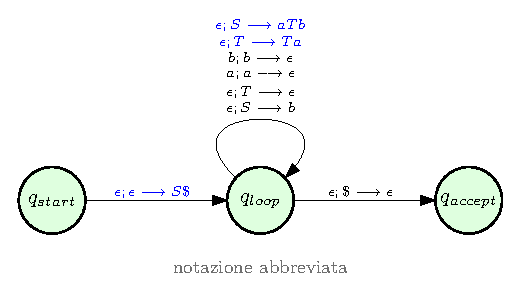
\includegraphics[width=0.65\textwidth ]{images/PDA2.2.eps}
\end{center}
\lemma{[$\impliedby$]}  Dato un PDA, esiste una CGF le cui stringhe generate sono il linguaggio del PDA.\acc 
\dimo{[$\impliedby$]} Sia $P=(Q,\Sigma,\Gamma,\delta,q_0,F)$ il PDA in questione. L'idea è quella di considerare,
 per ogni coppia di stati $p,q$ in $Q$, una variabile denotata $A_{pq}$ che genera tutte le stringhe 
 che permettono al PDA di passare da $p$ a $q$ lasciando la pila vuota, come nell'esempio in figura \ref{fig:dimopda1}.
 \begin{center}
    \begin{figure}[h!]
        \centering 
        \includegraphics[width=0.8\textwidth ]{images/dimopda1.eps}
        \caption{esempio}
        \label{fig:dimopda1}
    \end{figure}
\end{center}\sapbox{
\textbf{Forma Canonica} : Durante la dimostrazione, si assumerà che $P$ soddisfi certe proprietà, ossia che assuma una 
\textit{forma canonica}, tale forma non fa perdere di generalità alla dimostrazione in quanto ogni PDA 
può essere trasformato in un PDA in tale forma lasciando invariato il linguaggio che accetta. Un PDA è nella forma canonica 
se\begin{enumerate}
    \item Inizia con la pila vuota, ed termina la computazione sempre con la pila vuota 
    \item Ha un solo stato accettante $|F|=1$
    \item Il PDA ad ogni passo computazionale, non sostituisce mai un elemento della pila con un altro, o ne elimina 
    uno, o ne aggiunge uno, la sostituzione non avviene mai in un solo passo di computazione, formalmente, cambia la 
    definizione della funzione di transizione 
    $$\delta_1 : Q\times\Gamma_\epsilon\times\Sigma_\epsilon\rightarrow\mathcal{P}(Q\times\{\epsilon\})$$
    $$\delta_2 : Q\times\{\epsilon\}\times\Sigma_\epsilon\rightarrow\mathcal{P}(Q\times\Gamma_\epsilon)$$
    $$\delta = \delta_1\cup \delta_2$$
\end{enumerate}
È chiaro che ogni PDA può essere portato in tale forma, se ci sono più stati di accettazione, si creerà un nuovo stato 
alla quale tutti rimandano, rendendolo l'unico stato di accettazione. Quest'ultimo stato inoltre si occuperà 
di svuotare la pila automaticamente grazie agli $\epsilon$-archi. Inoltre, ogni arco che esegue una sostituzione 
nello stack sarà diviso in due archi che eseguono in sequenza un pop ed un push, facendo uso di uno stato 
intermedio.\begin{center}
    \includegraphics[width=1\textwidth ]{images/pdacanonico.eps}
\end{center}}
Bisogna definire le regole dela grammatica, la variabile iniziale $S$ sarà $A_{q_0q_{accept}}$, quindi per 
definizione $S$ genererà tutte le stringhe che accetta il PDA. L'insieme delle regole $R$ della grammatica $G$ sarà 
definito come segue \begin{itemize}
    \item Siano $p,q,r,s\in Q$, $u\in\Gamma$, $a,b\in\Sigma_\epsilon$, se $$ (r,u)\in\delta(p.a.\epsilon)\land  
    (q,\epsilon)\in\delta(s,b,u)$$ allora ci sarà la regola $$A_{pq}\longrightarrow aA_{rs}b $$\begin{center}\begin{figure}[h!]
        \centering
        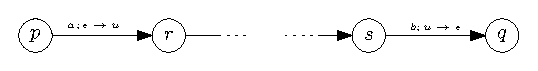
\includegraphics[width=0.8\textwidth ]{images/dimoPDACFG1.eps}
        \caption{situazione del PDA}
        \label{fig:dimoPDACFG1}
    \end{figure}\end{center}
    È ovvio che che si possa arrivare da $p$ a $q$ in tal modo, il carattere $a$ porta da $p$ ad $r$ (aggiungendo $u$), il 
    carattere $b$ porta da $s$ a $q$ (rimuovendo $u$), la variabile $A_{rs}$ deriva\footnote{
        con \textit{deriva}, si intende l'atto di generare tale stringa attraverso diverse produzioni, ossia la 
        chiusura transitiva della relazione di produzione, precedentemente denotata $\Rightarrow^*$
    } i caratteri che portano da $r$ ad $s$ con pila vuota.
    \item Per ogni tripla $p,q,r\in Q$ si pone la regola $A_{pq}\longrightarrow A_{pr}A_{rq}$. 
    \item Per ogni $p\in Q$, si pone la regola $A_{pp}\longrightarrow \epsilon$
\end{itemize}
La prova della dimostrazione segue dal fatto che $A_{pq}$ genera $x$ \textit{se e solo se} $x$ porta l'automa $P$ da 
$p$ a $q$ con pila vuota, ne segue che, se $S=A_{q_0q_{accept}}$ deriva $x$, allora $x\in L(P)$. Tale dimostrazione sarà 
suddivisa in due claim.\acc 
\claim{1} Se $A_{pq}$ deriva $x$, allora $x$ porta da $p$ a $q$ con pila vuota. \acc 
\dimo{ claim 1} Verrà dimostrato per induzione sul numero di produzioni di $x$ in $G$.\begin{itemize}
    \item \textbf{caso base} : $x$ è generata da una regola di $G$ per $k=1$ produzione, allora l'unica regola 
    che può generare $x$ è del tipo $A_{pp}\longrightarrow \epsilon$, allora $x=\epsilon$, e la stringa vuota porta 
    l'automa $P$ da $p$ a $p$ con pila vuota. 
    \item \textbf{ipotesi induttiva} : Per ogni $x$ generata da una regola di $G$ per $k>1$ produzioni, tale stringa 
    congiunga i due stati in questione lasciando la pila vuota. 
    \item \textbf{passo induttivo} : Supponiamo che $A_{pq}$ produca $x$ in $k+1$ produzioni, allora, data la definizione 
    delle regole di $G$, la regola in questione può essere di due tipi : \begin{itemize}
        \item La regola in questione è $A_{pq}\longrightarrow aA_{rs}b$, allora $x$ ha la forma $ayb$, ne consegue che 
        $A_{rs}$ deriva $y$ in al più $k$ passi, quindi, per ipotesi, la stringa $y$ porta l'automa $P$ dallo stato
        $r$ allo stato $s$ lasciando la pila vuota. Inoltre, per definizione delle regole è vero che 
        $$ (r,u)\in\delta(p,a,\epsilon)\land (q,\epsilon)\in\delta(s,b,u) \ \ \text{ per qualche }u\in\Gamma$$
        Quindi è chiaro che $x$ porti $P$ da $p$ a $q$ lasciando la pila vuota. 
        \item La regola in questione è $A_{pq}\longrightarrow A_{pr}A_{rq}$,, allora la stringa $x$ sarà del tipo 
        $yz$, quindi $A_{pr}$ deriva $y$, mentre $A_{rq}$ deriva $z$. Se $A_{pq}$ deriva $x$ in $k+1$ produzioni, allora 
        le derivazioni di $y$ e $z$ avvengono in al più $k$ produzioni, ma allora per ipotesi$$\begin{cases}
            y\text{ porta $P$ da $p$ a $r$ lasciando la pila vuota}\\ 
            z\text{ porta $P$ da $r$ a $q$ lasciando la pila vuota}
        \end{cases}\implies x=yz\text{ porta $P$ da $p$ a $q$ lasciando la pila vuota} $$
    \end{itemize}
    \hfill $\square$
\end{itemize}
\claim{ 2 } Se $x$ porta da $p$ a $q$ con pila vuota, allora $A_{pq}$ deriva $x$.\acc
\dimo{ claim 2} Verrà dimostrato per induzione sul numero di passi di computazione dell'automa $P$.\begin{itemize}
    \item \textbf{caso base} : L'automa compie 0 passi, la computazione inizia e finisce in $p$, l'input $x$ è quindi 
    la stringa vuota, siccome per definizione delle regole, $G$ ha la regola $A_{pp}\longrightarrow\epsilon$, allora 
    $A_{pp}$ deriva $x$. 
    \item \textbf{ipotesi induttiva} : Si ipotizza che per ogni computazione  di $k>0$ passi (che lasci vuota 
    la pila) da $p$ a $q$ con stringa in input 
    $x$, la regola $A_{pq}$ deriva $x$.  
    \item \textbf{passo induttivo} : Supponiamo che $x$ porti da $p$ a $q$ lasciando la pila vuota in $k+1$ passi di 
    computazione, precisamente, ci sono due possibili casi \begin{itemize}
        \item La pila è vuota solo negli stati $p$ e $q$, negli stati intermedi è stata riempita dal primo passo, e verrà 
        poi svuotata all'ultimo passo. Sia $u$, tale carattere inserito all'inizio e rimosso al termine, e sia $a$
        il simbolo che porta $p$ allo stato successivo $r$ (primo passo di computazione), e $b$ il simbolo che porta dal 
        penultimo stato $s$ a $q$ (ultimo passo di computazione), proprio come mostrato in figura \ref{fig:dimoPDACFG1}. Per 
        definizione, la grammatica $G$ contiene la regola $A_{pq}\longrightarrow aA_{rs}b$, quindi $x$ è del tipo 
        $ayb$. La variabile $A_{rs}$ deriva $y$, quindi $y$ porta da $r$ a $s$ lasciando la pila vuota con al più 
        $k-1$ passi. Ricapitolando\begin{itemize}
            \item $a$ porta da $p$ ad $r$ aggiungendo $u$
            \item $y$ porta da $r$ ad $s$ senza fare operazioni sulla pila 
            \item $b$ porta da $s$ a $q$ rimuovendo $u$
            \item $x=ayb$ porta da $p$ a $q$ lasciando la pila vuota 
            \item $A_{pq}$ deriva $x$.
        \end{itemize}
        \item La pila viene svuotata negli stati intermedi fra $p$ e $q$, sia $r$ lo stato in cui la pila 
        si svuota, essendo che la computazione da $p$ a $q$ richiede $k+1$ passi, allora le computazioni da 
        $p$ ad $r$ e da $r$ a $q$ richiederanno al più $k$ passi. Sia $x=yz$, $y$ porta da  $p$ ad $r$, e 
        $z$ porta da $r$ a $q$, per ipotesi $A_{pr}$ deriva $y$ e $A_{rq}$ deriva $z$, 
        ma allora, essendo che esiste la regola $A_{pq}\longrightarrow A_{pr}A_{rq}$ ne consegue che 
        $A_{pq}$ deriva $x=yz$.\begin{center}
            \includegraphics[width=0.8\textwidth ]{images/dimoPDACFG2.eps}
        \end{center}
    \end{itemize}
    \hfill $\square$
\end{itemize}
I due claim dimostrano il lemma $\impliedby$.\hfill $\blacksquare$\\
Essendo entrambi i lati dimostrati, il teorema sull'equivalenza fra PDA e CFG è dimostrato.
\subsection{Il Pumping Lemma per le Grammatiche Acontestuali} 
Il teorema presentato in questa sezione mostra che esistono anche dei linguaggi non acontestuali, ossia, per i quali non 
esiste alcuna grammatica che li genera. Un esempio di linguaggio acontestuale è il seguente 
$$ L=\{0^n1^n2^n\ | \ n\ge 1\}$$
Prima di presentare il teorema, è necessario introdurre il seguente fatto.\acc
\claim{} Sia $G$ una CFG in forma normale Chomsky, data la forma delle regole, ogni 
albero di derivazione di $G$ è binario, da ciò ne deriva che, preso un qualsiasi albero, se il cammino 
più lungo di tale albero è lungo $i$, allora  allora la stringa generata sarà 
lunga al più $2^{i-1}$.\acc 
\dimo{ claim } Si dimostra per induzione su $i$\begin{itemize}
    \item \textbf{caso base} : $i=1$, allora la derivazione è composta da una sola produzione, la stringa 
    è lunga 1, infatti $2^{i-1}=2^{1-1}=2^0=1$. 
    \item \textbf{ipotesi induttiva} : si assume sia vero per un generico $i>1$. 
    \item \textbf{passo induttivo} : si consideri un cammino lungo $k=i+1 =  (i>1)+1 \ge 3$, la prima regola applicata 
    deve essere necessariamente del tipo $$S\longrightarrow BC$$ i sotto alberi generati da $B$ e $C$ hanno il 
    cammino più lungo (denominato da ora in poi \textit{altezza}) grande al più $i$, generano quindi stringhe 
    lunghe al più $2^{-1}$, quindi $S$ genera stringhe lunghe al più $2\cdot 2^{i-1}=2^i=2^{k-1}$.\hfill$\blacksquare$
\end{itemize}
\teo{( Pumping Lemma per le CFG )} : Sia $L$ un linguaggio acontestuale, allora esiste un numero $p$ tale che, presa 
una qualsiasi stringa $w$ lunga almeno $p$, ($|w|\ge p$), esiste una sua suddivisione $$w=uvxyz$$ tale che\begin{enumerate}
    \item $\forall i\ge 0 \ \ \ uv^ixy^iz\in L$
    \item $|vy|>0$
    \item $|vxy|\ge p$
\end{enumerate}
\dimo{( Pumping Lemma per le CFG )} Sia $G=(V,\Sigma, R, S)$ la CFG associata ad $L$, ossia $L(G)=L$, si assume che $G$ sia in forma 
normale Chomsky (senza perdita di generalità), quindi ogni suo albero di derivazione sarà binario. Sia $m=|V|$ il numero 
di variabili distinte di $G$, identifichiamo come \textit{pumping} il numero $p=2^m$. Sia $w$ una generica stringa tale 
che $|w|\ge p = 2^m$, allora $w$ avrà un albero di derivazione di altezza almeno $m+1$, ed il numero di nodi 
nell'albero sarà almeno $m+2$, di cui 1 nodo è necessariamente un terminale, e gli altri $m+1$ sono variabili.\acc 
Sia $w=uvxyz$, siccome le variabili distinte sono $m$, esiste una variabile $A_i$ che si ripete nell'albero, in particolare \begin{itemize}
    \item L'albero con radice $A_i$ genera $vxy$
    \item L'albero con radice $A_j=A_i$ genera $x$
\end{itemize}
Mentre $u$ e $z$ sono generate nella derivazione da $S$ ad $A_i$.\begin{center}
    \includegraphics[width=0.4\textwidth ]{images/alberoDer1.eps}
\end{center}
Siccome $G$ è in forma normale, un sotto albero contiene, o un singolo terminale, o due variabili. Quindi, essendo che il 
sotto albero di $A_i$ non può essere un terminale, avendo $A_j$, sarà composto da due variabili. 
$$A_i\longrightarrow BC\in R $$
Una delle due variabili fra $B$ e $C$ genererà $A_j$ che a sua volta deriverà $x$. L'altra variabile deriverà 
$vy$, quindi $vxy\ne x$, ciò implica che necessariamente $|vy|>0$ (punto $(ii)$ dimostrato).\acc 
Essendo che il cammino più lungo nell'albero ha lunghezza $m+1$, le stringhe generate avranno lunghezza 
minore o uguale a $2^{(m+1)-1}=2^m=p$, quindi $|vxy|\ge p$  (punto $(iii)$ dimostrato).\acc 
Le variabili $A_i$ e $A_j$ possono essere sostituite nell'albero di computazione.
\begin{center}
    \includegraphics[width=0.85\textwidth ]{images/alberoDer2.eps}
\end{center}
In generale, è chiaro come $\forall i \ uv^ixy^iz\in L$. (punto $(i)$ dimostrato), la dimostrazione del 
teorema è completa.\hfill$\blacksquare$
\subsection{Esercizi ed Ultime Proprietà sulle CFG}
In questa sezione verrà utilizzato il pumping lemma per dimostrare che alcuni linguaggi non sono acontestuali.
\subsubsection{Esercizio 1}
Si consideri il linguaggio 
$$ L=\{0^n1^n2^n \ | \ n \ge 1 \}$$
Tale linguaggio non è acontestuale, non esiste nessuna CFG che lo genera. Per assurdo, si assuma che 
$L$ sia acontestuale, allora $\exists p$ tale che, per ogni stringa $w\in L$ di lunghezza al più 
$p$, valgono le condizioni del pumping lemma. \acc 
Si prende in esame la stringa $w=0^p1^p2^p$, bisogna considerare tutte le scomposizioni di $w$ del tipo\begin{itemize}
    \item $w=uvxyz$ con  
    \item $|vy|>0$
    \item $|vxy|\le p$
\end{itemize}
$$ w=\smash{\underbrace{00\dots 0}_{p\ \text{volte}}} \
\smash{\underbrace{11\dots 1}_{p\ \text{volte}}} \
\smash{\underbrace{22\dots 2}_{p\ \text{volte}}}$$
\\Se la stringa $vxy$ è lunga al più $p$ conterrà 1 oppure 2 caratteri distinti, dato che, se contenesse 3 caratteri distinti (sia 0 che 1 che 2 ) allora 
per costruzione di $w$ sarebbe lunga più di $p$. Si consideri il punto $(1)$ del pumping lemma, preso $i=0$ la stringa 
$$ \hat w=uv^0xy^0z$$
Deve essere contenuta in $L$. Siccome la stringa $vxy$ per definizione non era vuota, la stringa $\hat w = uxz$ 
avrà un numero di elementi minore di $w$ dato che $v$ ed $y$ sono state rimosse ed insieme erano composte da 
almeno 1 carattere. 
\acc 
La rimozione di $vy$ comporta il cambio del numero di occorrenze di 1 (oppure 2) simboli in $\hat w$ rispetto a 
$w$, quindi $\hat w$ avrà 1 (oppure 2) simboli le cui occorrenze differiscono dal/dai restante/restanti, ma allora 
non è del tipo $0^n1^n2^n, \ \ n \ge 1$, quindi non è in $L$, ma allora non è vero che 
$L$ è acontestuale.
\subsubsection{Esercizio 2}\label{es2}
Si consideri il linguaggio 
$$ L=\{ww \ | \  w\in\{0,1\}^* \}$$
Tale linguaggio non è acontestuale, non esiste nessuna CFG che lo genera. Per assurdo, si assuma che $L$ sia 
acontestuale, allora $\exists p$ tale che, per ogni stringa $w\in L$ di lunghezza al più 
$p$, valgono le condizioni del pumping lemma. \acc Si considera la stringa $$ w=0^p1^p0^p1^p$$ di cardinalità $|w|=4p$, 
bisogna considerare ogni possibile modo di scomporre la stringa, come prima cosa, si individuano le seguenti sezioni 
nella stringa\begin{center}
    \includegraphics[width=0.6\textwidth ]{images/sezioniStringa4p.eps}
\end{center}
La stringa può essere scomposta in diversi modi\begin{itemize}
    \item \textit{caso 1} : $vxy$ non si trova a cavallo fra i confini e non si trova a cavallo nel mezzo, è 
    quindi confinata fra una delle 4 metà della stringa, è quindi composta di soli 0 oppure di soli 1. Secondo il punto 
 $(1)$ del pumping lemma, preso $i=2$ si ha la stringa $$ \hat w = uv^2xy^2z$$
ma allora $\hat w$ non appartiene ad $L$. 
\item \textit{caso 2} : $vxy$ si trova a cavallo fra uno dei due confini, ma non tocca il mezzo. Si considera $i=0$ : 
$$ \hat w = uv02xy^0z=uxz$$
eliminando $vy$, si crea un "buco" rispetto alla stringa originale, tale buco ha dimensione 
al più $p$, essendo che una delle due metà della stringa cambia, il mezzo si sposta, supponiamo che $vxy$ si trovava sul confine 
destro (la dimostrazione è analoga al sinistro), allora il centro si sposterà verso destra di $\ge p$ posizioni, e la metà destra della 
stringa terminerà necessariamente con un 1, ma la metà sinistra terminerà necessariamente con uno zero, quindi le due metà 
non sono uguali e $\hat w\notin L$. 
\item \textit{caso 3} : $vxy$ si trova a cavallo sul mezzo ma non oltrepassa alcun confine. Si considera, preso $i=0$
$$ \hat w = uxz$$ 
In tal modo, la seconda e la terza sezione di $w$ verrà modificata, ed una delle due parti avrà meno di $p$ caratteri 
$$  w = \smash{\underbrace{00\dots 0}_{p\ \text{volte}}} \
\smash{\underbrace{11\dots 1}_{p\ \text{volte}}} \
\smash{\underbrace{00\dots 0}_{p\ \text{volte}}} \
\smash{\underbrace{11\dots 1}_{p\ \text{volte}}} $$ 
\\
$$ \hat w = \smash{\underbrace{00\dots 0}_{p\ \text{volte}}} \
\smash{\underbrace{11\dots 1}_{k\ \text{volte}}} \
\smash{\underbrace{00\dots 0}_{j\ \text{volte}}} \
\smash{\underbrace{11\dots 1}_{p\ \text{volte}}} $$\\ $$k\ne p\lor j\ne p $$
\\Ma allora $\hat w \notin L$.
\end{itemize}
Durante dimostrazioni di questo tipo può risultare utile l'applicazione di una proprietà delle CFG, ossia la loro 
\textbf{chiusura per concatenazione}, siano $G_1=(V_1,\Sigma, R_1, S_1)$ e $G_2=(V_2,\Sigma, R_2, S_2)$ due CFG, la grammatica 
$G=(V_1\cup V_2,\Sigma, R, S)$ dove \begin{itemize}
    \item $S$ è un nuovo stato 
    \item $R=R_1\cup R_2\cup\{S\rightarrow S_1S_2\}$
\end{itemize}
é ancora una CFG.
\acc 
Differentemente, le CFG non sono chiuse per intersezione, basta dare un singolo contro esempio per dimostrare la tesi, si 
considerino i seguenti linguaggi 
$$ \begin{matrix}
    L_1=\{0^n1^n2^i \ | \ n\ge 0\land i\ge 0\}\\ 
    L_2=\{0^k1^n2^n \ | \ n\ge 0\land k\ge 0\}
\end{matrix}$$
Entrambi i linguaggi sono acontestuali, infatti sono generati dalle regole 
$$ R_1=\begin{cases}
    S\longrightarrow S_1S_2\\ 
    S_1\longrightarrow0S_1 1|\epsilon\\ 
    S_2 \longrightarrow 2S_2|\epsilon
\end{cases} \ \ \ \ \ \ \ \ R_2=\begin{cases}
    S\longrightarrow S_1S_2\\ 
    S_1\longrightarrow0S_1 |\epsilon\\ 
    S_2 \longrightarrow 1S_22|\epsilon
\end{cases}$$
L'intersezione dei due linguaggi $L=L_1\cup L_2 = \{0^n1^n2^n \ | \ n\ge 0\}$ sappiamo essere un linguaggio acontestuale, 
quindi le CFG \textbf{non sono chiuse per intersezione}.
\subsubsection{Esercizio 4}
Si consideri il seguente linguaggio $$ L=\{a,b\}^* \ \backslash \ \{ww\ | \ w\in\{a,b\}^*\}$$
Comprende tutte le stringhe che non possono essere scritte come una stessa stringa ripetuta due volte. Nell'esercizio 
\ref{es2} si è visto 
che il complementare di $L$, non è un linguaggio acontestuale, si vuole dimostrare che invece $L$ lo è. Sicuramente, 
tutte le stringhe di cardinalità dispari saranno in $L$. Le regole che generano il linguaggio sono le seguenti$$ 
R=\begin{cases}
    S\longrightarrow A|B|AB|BA\\ 
    A\longrightarrow a|aAa|aAb|bAa|bAb 
    B\longrightarrow b|aBa|aBb|bBa|bBb 
\end{cases}
$$\begin{itemize}
    \item $A$ genera le stringhe dispari con una $a$ al centro
    \item $B$ genera le stringhe dispari con una $b$ al centro
\end{itemize}
\dimo{} : Si vuole dimostrare che le stringhe di lunghezza pari generate da $R$ sono in $L$. Si dimostreranno entrambi i 
versi.\acc 
\boxedMath{$\implies$} Se $x\in L$, allora $S\Rightarrow^* x$. Se $x\in L$, allora esiste almeno una lettera che si differenzia fra le due sotto stringhe di eguale 
lunghezza che compongono $x$, sia $n=|x|$
$$\exists \ i \ | \ x_i\ne x_{\nicefrac{n}{2}+1} $$
$x$ può essere scritta come unione di due 
stringhe di lunghezza dispari $x=uv$. Si pongono \begin{itemize}
    \item $u=x_1x_2\dots x_{2i-1}$
    \item $v=x_{2i}x_{2i+1}\dots x_n$
\end{itemize}
$S\longrightarrow AB$ e $A\longrightarrow u \land B\longrightarrow v \implies S\Rightarrow^* x$.\acc 
\boxedMath{$\impliedby$} Se $S\Rightarrow^* x$ allora $x\in L$. 
Siccome $|x|=n=0\mod 2$, può essere generata a partire da $S\longrightarrow AB$ oppure $S\longrightarrow BA$, si suppone che 
sia generata dalla prima (il procedimento è analogo), 
allora $x=uv$ con $u\ne v$ e \begin{itemize}
    \item $A\Rightarrow^* u$
    \item $B\Rightarrow^* v$
\end{itemize}
Sia $|u|=l$ e $|v|=n-l$, le lettere centrali di $u$ e $v$ sono \begin{itemize}
    \item $u_{\frac{l+1}{2}}$
    \item $v_{\frac{n-2+1}{2}}$
    \item dove $u_{\frac{l+1}{2}}\ne v_{\frac{n-2+1}{2}}$
\end{itemize}
Scrivendo le lettere in funzione di $x$ si ha 
$$ u_{\frac{l+1}{2}}=x_{\frac{l+1}{2}} \ \ \ \  \  v_{\frac{n-2+1}{2}}=x_{\frac{n+l+1}{2}}
$$
\redText{dimostrazione non completa}
\chapter{Calcolabilità}
\section{Macchina di Turing}
Esistono linguaggi che nessuna CFG può accettare, si vuole estendere il modello di calcolo ad uno più 
potente. Negli anni 30' del ventesimo secolo fu introdotta la \textbf{Macchina di Turing} (alla quale ci 
riferiremo come TM), estendendo gli automi dandogli una memoria illimitata, tale modello è una semplice 
astrazione dei calcolatori odierni, e corrisponde alla nozione di algoritmo.\subsubsection{Caratteristiche di una TM}\begin{itemize}
    \item Una TM possiede un \textit{nastro di lavoro}, rappresenta una memoria (illimitata) sulla quale il modello 
    può scrivere dei caratteri. 
    \item Una \textit{testina di lettura} che identifica la precisa posizione attuale sul nastro, che può spostarsi 
    a destra o a sinistra. 
    \item Vi sono poi degli \textit{stati di accettazione} (la stringa in input è accettata dalla TM) e degli 
    \textit{stati di rifiuto} (la stringa in input è rifiutata dalla TM). Quando la TM passa su uno stato di rifiuto, 
    la computazione è immediatamente terminata. 
    \item È possibile che per alcuni input una TM entri in uno stato di \textit{loop} in cui non termina.
\end{itemize}
\defi{(Turing Machine)} Una TM $T=(Q,\Sigma,\Gamma,\delta,q_0,q_{acc},q_{rej})$ è una tupla tale che \begin{itemize}
    \item $Q$ è l'insieme degli stati 
    \item $\Sigma$ è l'alfabeto delle stringhe in input 
    \item $\Gamma$ è l'insieme dei caratteri che possono essere scritti sul nastro, solitamente $\Sigma\subseteq \Gamma$. Inoltre 
    in $\Gamma$ vi è sempre un carattere speciale $\blank$ (denominato "blank") che rappresenta il carattere vuoto.
    Inoltre $\blank\notin\Sigma$.
    $\delta$ è la funzione di transizione definita $$ \delta : Q\times \Gamma \rightarrow Q\times \Gamma \times \{L,R\}$$
    L'insieme $\{L,R\}$ rappresenta i possibili spostamenti della testina a sinistra o a destra
    \item $q_0$ è lo stato iniziale 
    \item  $q_{acc}$ è lo stato (unico) di accettazione 
    \item $q_{rej}$ è lo stato (unico) di rifiuto 
\end{itemize}
Canonicamente, la configurazione iniziale di una TM prevede l'intera stringa in input contenuta nel nastro, seguita 
dal carattere $\blank$.\begin{center}
    \includegraphics[width=0.7\textwidth ]{images/turingMachine.eps}
\end{center}
Una TM computa la stringa in input seguendo le regole definite dalla $\delta$, come per gli automi, per una 
TM è defintia la configurazione ad un certo passo nella configurazione, essa determina il contenuto del nastro, la 
posizione della testina, e lo stato attuale. Una configurazione si denota $$ uqav$$ dove \begin{enumerate}
    \item $u,v\in\Gamma^*$
    \item $q\in Q$
    \item $uav$ è il contenuto del nastro, $a\in\Gamma$ è il carattere su cui si trova la testina.
\end{enumerate}
Data in input una stringa $w$, la configurazione iniziale sarà $q_0w$. Si può rappresentare graficamente una 
configurazione come segue\begin{center}\begin{figure}[h!]
    \centering 
    \includegraphics[width=0.8\textwidth ]{images/confTM.eps}
    \caption{la testina è sul carattere $w_i$ e lo stato attuale è $q$}
\end{figure}
\end{center}
Per definire il concetto di accettazione, bisogna stabilire la relazione di \textit{produzione} :
 $$\begin{matrix}
    uaq_ibv \text{ produce }uq_jacv \\ \text{se e solo se}\\ 
    \delta(q_i,b)=(q_j,c,L)
 \end{matrix} $$
Vuol dire che la TM, nello stato $q_i$, leggendo con la testina il carattere $b$ si sposta a sinistra. Può 
essere analogamente definito per lo spostamento a destra.
$$\begin{matrix}
    uaq_ibv \text{ produce }uacq_jv \\ \text{se e solo se}\\ 
    \delta(q_i,b)=(q_j,c,R)
 \end{matrix} $$
 Diremo che una TM \textbf{accetta} $w$ se e solo se esiste una sequenza di configurazioni 
 $$ C_1\rightarrow C_2\rightarrow C_3\dots\rightarrow C_k$$
 dove \begin{itemize}
    \item $C_1=q_0w$ 
    \item $\forall i \ \ \ C_i$ produce $C_j$
    \item lo stato della configurazione $C_k$ è lo stato accettante $C_k=uq_{acc}av$
 \end{itemize}
 \defi{(Riconoscibilità)} Un linguaggio $L$ è \textbf{turing riconoscibile} se esiste una TM $M$ che 
 \textit{accetta} ogni sua stringa, si dice che $L$ è il linguaggio di $M$.\acc 
 Se una TM deve computare una stringa che non è nel suo linguaggio, può \begin{itemize}
    \item rifiutare 
    \item andare in loop
 \end{itemize}
 Una TM $M$ per cui, data una qualsiasi stringa, non vai mai in loop, viene detta \textbf{decisore}.\acc 
 \defi{(Decidibilità)} Un linguaggio $L$ è \textbf{turing decidibile} se esiste una TM $M$ che è un 
 decisore per $L$, ossia, per ogni sua stringa, non va mai in loop. Si dice che $M$ \textit{decide} $L$.\acc 
Data una TM $M$ si hanno gli insiemi \begin{itemize}
    \item $L(M)=\{w\in\Sigma^* \ | \ M\text{ accetta }w \}$
    \item $R(M)=\{w\in\Sigma^* \ | \ M\text{ rifiuta }w \}$
    \item Generalmente $L(M)\cup R(M)\subseteq \Sigma^*$
    \item Se $L(M)\cup R(M)= \Sigma^*$ allora $M$ è un decisore.
 \end{itemize}
 Un linguaggio che non ha decisori \textit{non è decidibile}, la definizione di decidibilità stabilisce i limiti della 
 computabilità, esistono infatti dei linguaggi (astrando, dei problemi) che non possono essere decisi (non possono essere 
 risolti), ciò si lega inevitabilmente con i \textit{teoremi di incompletezza} di Gödel, esisteranno sempre 
 delle proposioni per cui è \textit{impossibile} stabilire se sono vere o false. 
 \subsection{Esempi di TM}
 Le TM verranno rappresentato in maniera compatta sottoforma di grafi proprio come per gli automi.
 \begin{center}
	\begin{tabular}{>{\centering\arraybackslash}m{3in}>{\arraybackslash}m{3in}}
        \begin{tikzpicture} [node distance = 5cm, on grid, auto]
            \node (q1)[state, left] {$q_1$};
            \node (q2)[state, right = of aperta] {$q_2$};
            \path [-stealth, thick]
            (q1) edge  node {$a\rightarrow b,R$}   (q2);
        \end{tikzpicture} & Il grafo rappresentato in figura descrive la seguente situazione : Se la TM si trova 
        nello stato $q_1$, e la testina si trova sul carattere $a$, allora si sostituisce il carattere 
        $a$ nel nastro con il carattere $b$, si sposta la testina a destra (se al posto di $R$ ci fosse 
        stato $L$ si sarebbe andati a sinistra) e la TM si sposta nello stato $q_2$.
		\\
	\end{tabular}
\end{center}
\subsubsection{Esempio 1}
Si consideri il seguente linguaggio $L=\{01^*0\}$. La TM che decide $L$ è la seguente\begin{center}
    \begin{tikzpicture} [node distance = 4cm, on grid, auto]
        \node (q0)[state, initial, left] {$q_0$};
        \node (B)[state, right = of q0] {$B$};
        \node (C)[state, right = of B] {$C$};
        \node (rej)[state, below = of B] {$q_{rej}$};
        \node (acc)[state,accepting, below = of C] {$q_{acc}$};
        \path [-stealth, thick]
        (B) edge [loop above]  node {$1\rightarrow y, R$}()
        (q0) edge  node {$0\rightarrow x,R$}  (B)
        (q0) edge [bend right]  node[left] {$\begin{matrix}\\1\rightarrow 1,R \ \ \\\blank\rightarrow \blank,R\ \ \end{matrix}$}  (rej)
        (B) edge  node {$0\rightarrow x,R$}  (C)
        (C) edge  node {$\blank\rightarrow \blank,R$}  (acc)
        (C) edge  node {$\begin{matrix}1\rightarrow 1,R\\0\rightarrow 0,R\end{matrix}$}  (rej)
        (B) edge  node {$\blank\rightarrow \blank,R$}  (rej);
    \end{tikzpicture}
\end{center}
Esempio di computazione su una stringa di $L$:$$ 
\begin{matrix}
    \bar 0 1 1 1 0 \blank & & x\bar 1 1 1 0 \blank&& xy\bar 1 1 0 \blank\\ xyy\bar 10\blank & & xyyy\bar 0\blank && xyyyx\bar \blank
\end{matrix} 
$$
\subsubsection{Esempio 2}\label{esempioTM2}
Si consideri il seguente linguaggio $L=\{0^n1^n \ | \ n\ge 0\}$. La TM che decide $L$ è la seguente (stato di 
rifiuto omesso)\begin{center}
    \begin{tikzpicture} [node distance = 3cm, on grid, auto]
        \node (A)[state, initial, left] {$A$};
        \node (B)[state, right = of A] {$B$};
        \node (C)[state, right = of B] {$C$};
        \node (D)[state, below = of A] {$D$};
        \node (acc)[state,accepting, below = of D] {$q_{acc}$};
        \path [-stealth, thick]
        (B) edge [loop below]  node {$\begin{matrix}y\rightarrow y,R\\0\rightarrow 0,R\end{matrix}$}()
        (D) edge [loop right]  node {$y\rightarrow y,R$}()
        (C) edge [loop right]  node {$\begin{matrix}y\rightarrow y,L\\0\rightarrow 0,L\end{matrix}$}()
        (A) edge  node[below] {$0\rightarrow x,R$}  (B)
        (A) edge [bend right] node[left] {$\blank\rightarrow \blank,R$}  (acc)
        (A) edge  node {$y\rightarrow y,R$}  (D)
        (D) edge  node {$\blank\rightarrow \blank,L$}  (acc)
        (B) edge  node[below] {$1\rightarrow y,L$}  (C)
        (C) edge [bend right] node[above] {$x\rightarrow x,R$}  (A);
    \end{tikzpicture}
\end{center}
Nel capitolo precedente si è visto come il linguaggio $L=\{0^n1^n2^n \ | \ n\ge 0\}$  non è acontestuale, 
è possibile computarlo tramite le TM, de facto, basterà unire 2 TM che si comportino come 
quella vista nell'esempio \ref{esempioTM2}, infatti nella prima computazione si occuperà di controllare 
che la stringa in input abbia i primi $2n$ caratteri del tipo $0^n1^n$.$$
00\dots 0 \  \ 11\dots 1 \ \ 22\dots 2  \ \ \text{ viene trasformata } \ \ xx\dots x \ \ yy\dots y \ \ 22\dots 2$$
La seconda TM si occuperà di controllare se gli ultimi $2n$ caratteri sono del tipo $y^n2^n$. $$
xx \dots x \ \ yy\dots y\  \ 22\dots 2 \ \ \text{ viene trasformata }  \  \ xx\dots x \ \  xx \dots x  \ \ yy \dots y
$$
Senza perdita di generalità, è possibile astrarre le TM considerano due nuovi modelli equivalenti\begin{itemize}
    \item \textbf{TM multinastro}
    \item \textbf{TM non deterministica}
\end{itemize}
Prima di introdurli, si consideri il seguente esempio di 
astrazione di una TM, ossia di una macchina che, ad ogni passo di 
computazione, piuttosto che spostarsi necessariamente a destra o 
a sinistra, può rimanere ferma, la denominiamo STM. \acc 
La definiamo $M'$, e la sua funzione di transizione sarà del tipo 
$$ \delta':Q\times\Gamma \rightarrow Q\times\Gamma\times \{L,R,S\}$$
Dove $S$ (che sta per 'stay') indica l'azione del restare fermi senza 
muovere la testina.\acc 
\prop{} Per ogni STM esiste una TM classica equivalente. \acc 
\dimo{} ,Sia $M'$ la STM, l'idea è quella di considerare una TM $M$ 
che gestisca le transizioni di stato in cui la testina 
non si muove, a tal scopo, basta simulare tale azione tramite 
una sequenza di 2 movimenti che fanno uso di uno stato ausiliario $q_s$. 
\begin{center}
    $ \delta'(q,a)=(p,b,S)$
    \\ è equivalente alle azioni \\ 
    $\begin{cases}
        \delta(q,a)=(p,q_s,L)\\ 
        \delta(q_s,*)=(p,*,R)
        
    \end{cases}$
\end{center}
dove $*$ rappresenta un qualsiasi elemento di $\Gamma$.
\subsection{TM multi nastro}
Introduciamo la macchina di Turing con più nastri, che verrà 
denotata MTM, 
sia $k$ il numero di nastri, ogni nastro avrà 
una testina proprietaria, uno stato sarà quindi rappresentato 
dalle stringhe scritte su tutti e $k$ i nastri, e la relativa 
posizione delle testine. \acc 
La funzione di transizione prenderà le decisioni valutando le posizioni 
ed il valore di tutte le testine 
$$ \delta : Q\times\Gamma^k\rightarrow Q\times\Gamma^k\times \{L,R\}^k$$
\teo{(MTM$\equiv$TM)} Per ogni MTM esiste una TM equivalente.\acc 
\dimo{} La dimostrazione, piuttosto che formale, mostrerà la costruzione di una 
TM che si comporta come la generica MTM.\acc 
Sia $MM$ la macchina multi nastro, ed $M$ la macchina classica 
 che deve simularla, si introduce un nuovo carattere $\#\notin \Gamma$
 che verrà utilizzato nel nastro di $M$ come separatore per i 
differenti nastri originari di $MM$.\begin{center}
    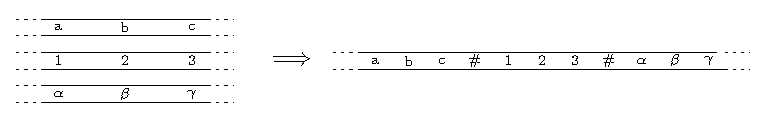
\includegraphics[width=\textwidth ]{images/multinastro.eps}
\end{center}
Per simulare le $k$ testine, si implementa la possibilità per $M$ 
di \textit{marcare} i caratteri (in tal caso, con un punto come 
apice). I caratteri marcati indicano che la testina è posta su di essi. Sia $\Gamma'$ l'alfabeto dei nastri di $MM$, e 
$\Gamma$ l'alfabeto del nastro di $M$.
$$\forall a\in\Gamma', \ \ \ \exists \dot{a} \in\Gamma$$
Si descrive ora la computazione di $M$, data una stringa 
in input $w$ la configurazione iniziale è la seguente: 
$$\#\dot{w_1}w_2w_3\dots,w_n\# 
\smash{\underbrace{\dot{\blank}\#\dot{\blank}\dots \#\dot{\blank}}_{k-1\ \text{volte}}}
$$
\\ 
Nel \textit{passo di computazione}, 
si scansiona una prima volta il nastro 
partendo dal primo simbolo $\#$, leggendo tutti i 
caratteri marcati, considerando poi la funzione di 
transizione, si esegue una seconda scansione aggiornando i 
valori delle testine (le marcature dei caratteri) ed il contenuto 
dei $k$ caratteri in questione. Se la testina su uno dei nastri deve 
spostarsi su $\#$, allora $M$ sposta il contenuto dell'intero nastro a destra di 1 posizione.\acc 
\textbf{Corollario} : $L$ è turing riconoscibile/decidibile se e solo se esiste una MTM che lo riconosce/decide.
\subsection{TM non deterministiche}
Si arricchisce il modello della macchina di turing introducendo il non determinismo, denotandolo NTM, la funzione di transizione cambia definizione 
$$ \delta : Q\times\Gamma \rightarrow \mathcal{P}(Q\times \Gamma \times \{L,R\})$$
Per ogni input si diramano più vie di computazione, una NTM accetta una stringa in input se almeno un ramo di computazione è accettante.\acc 
\teo{(NTM$\equiv$TM)} Per ogni NTM esiste una TM equivalente.\acc 
\dimo{} La dimostrazione, piuttosto che formale, mostrerà la costruzione di una 
TM che si comporta come la generica NTM.\acc Sia $N$ la NTM in questione, e sia $M$ la TM classica che la vuole 
simulare. $M$, per essere equivalente, dovrà esplorare ogni ramo di computazione, precisamente, deve esplorarlo in altezza. L'esplorazione in profondità in presenza di un loop su un ramo di computazione, comporterà il loop su $M$, anche se l'originaria $N$ aveva uno stato accettante su un differente ramo. \begin{center}
    \includegraphics[width=0.3\textwidth ]{images/loopEAccettante.eps} 
\end{center}
\textbf{Idea algoritmica} : $M$ utilizzerà 3 nastri\begin{enumerate}
    \item il primo nastro conterrà la stringa in input che non verrà modificata (il riferimento va mantenuto)
    \item il secondo nastro sarà il nastro di lavoro che verrà modificato per esplorare un cammino emulando la NTM.
    \item il terzo nastro conterrà l'indirizzo del nodo 
    dell'albero che si sta esplorando.
\end{enumerate}
Nell'$i$-esimo step, identificato da una tripla 
$$ (M,w,i)$$
usando l'input del primo nastro si percorre il ramo simulando $N$, se viene trovato uno stato accettante, 
$M$ accetta, altrimenti si incremente l'indice $i$
 e si ripercorre.
 \begin{itemize}
    \item Se un ramo di $N$ è accettante, $M$ accetta 
    \item Se ogni ramo di $N$ rifiuta, $M$ rifiuta 
    \item Se almeno un ramo di $N$ va in loop, e nessun 
    ramo accetta, $M$ va in loop.
 \end{itemize}
 \begin{quote}
    Se una NTM è un decisore, tutti i cammini hanno lunghezza finita
 \end{quote}
 \hfill$\blacksquare$
 \subsection{L'Enumeratore}
 L'enumeratore è un modello (in particolare, una variante di una TM) capace di generare un preciso insieme di stringhe, in un qualsiasi ordine e con eventuali ripetizioni, in particolare, per ogni linguaggio turing-riconoscibile, esiste un enumeratore che lo genera.\acc
Un enumeratore è una TM che "stampa" delle stringhe, eventualmente, infinite.\acc 
\teo{} Un linguaggio è turing riconoscibile se e solo se esiste un enumeratore che lo genera.\acc 
\dimo{} Si dimostrano separatamente le due direzioni.\acc 
\boxedMath{$\impliedby$} Dato un enumeratore $E$, definiamo una TM $M$ come segue (sia $w$ l'input)\begin{itemize}
    \item Si esegue $E$, se stampa una stringa, si confronta con $w$
    \item Se $w$ è uguale ad una stringa stampata da $E$, allora $M$ accetta.
\end{itemize}
\boxedMath{$\implies$} Sia $M$ una TM, si considera un enumeratore $E$ che deve 
stampare $L(M)$. Sia $\Sigma$ l'alfabeto di 
$L(M)$, identifichiamo come segue 
$$ \Sigma^*=\{\epsilon,s_1,s_2\dots\}$$
la lista di tutte le possibile stringhe su tale alfabeto. $E$ sarà definito come segue 
\begin{itemize}
    \item Si ripetono i passi per $i=1,2\dots$\begin{itemize}
        \item Si esegue $M$ per $i$ passi su ogni input $s_1,s_2\dots s_i$
        \item Se una qualsiasi computazione su $s_j$ accetta, $E$ stampa 
        $s_j$
    \end{itemize}
\hfill$\blacksquare$\end{itemize}\flowerLine 
\section{Decidibilità dei Linguaggi}
Come esistono linguaggi non regolari e linguaggi non acontestuali, risulta naturale porsi la domanda : Esistono dei linguaggi non turing riconosibili? Il modello della TM corrisponde al concetto di algoritmo, un linguaggio non riconoscibile corrisponde ad un problema che \textit{nessun} algoritmo può risolvere.\acc 
Una TM può ricevere in input un qualsiasi oggetto matematico, come un polinomio, un DFA, o direttamente un'altra TM, è importante che tale oggetto $O$, venga \textbf{codificato} in binario, denotandolo $<O>$ prima di essere computato dalla TM.\acc 
Vediamo come prima cosa un esempio di linguaggio decidibile, si consideri 
$$A_{DFA}=\{<D,w>\ |\ D \in DFA \land w\in L(d)\}$$
con $D\in DFA$ si indica che $D$ è un DFA. \acc 
\prop{} $A_{DFA}$ è decidibile. \acc 
\dimo{} Si vuole costruire un decisore per $A_{DFA}$, la TM in questione avrà il seguente comportamento\begin{enumerate}
    \item Su input $<D,w>$ interpreta $D$ come un DFA e $w$ come stringa, se non riconosce l'input, rifiuta 
    \item Simula l'esecuzione di $D$ con input $w$
    \item Se $D$ accetta $w$, allora la TM accetta, altrimenti rifiuta
\end{enumerate}
\hfill $\blacksquare$\acc 
In maniera simile, si può dimostrare che anche  $A_{NFA}=\{<N,w>\ |\ D \in NFA \land w\in L(d)\}$ è decidibile, utilizzando una TM non deterministica, oppure, si potrebbe trasformare l'input in un DFA ed eseguire l'algoritmo appena trattato. \acc  
Si consideri il linguaggio 
$$ E_{DFA}=\{<D>\ | \ D\in DFA \land L(D)=\emptyset\}$$
Ossia di tutte le codifiche di DFA che hanno linguaggio vuoto, ossia che non accettano nessuna stringa. \acc 
\prop{} $E_{DFA}$ è decidibile. \acc 
\dimo{} La TM che deciderà il linguaggio codificherà il DFA come un grafo, in gli stati sono i nodi, e vi è un arco da un nodo ad un altro solo se esiste una transizione fra i due stati. In particolare la TM seguirà il seguente comportamento\begin{enumerate}
    \item marca lo stato iniziale, ed inizia a fare una passeggiata sul grafo 
    \item marca ogni stato raggiungibile 
    \item se almeno uno stato di accettazione è marcato, la TM rifiuta, altrimenti accetta\hfill $\blacksquare$
\end{enumerate}
Un altro esempio interessante è il seguente 
$$ EQ_{DFA}=\{<D_1,D_2>\ | \ D_1,D_2\in DFA\land L(D_1)=L(D_2)\}$$
L'insieme delle coppie (codificate) di DFA che accettano lo stesso linguaggio.\acc 
\prop{} $EQ_{DFA}$ è decidibile. \acc 
\dimo{} Dati due DFA si definisce l'operatore di  differenza simmetrica $\Delta$ come segue 
$$ L(D_1)\Delta L(D_2)= (L(D_1)\cap \overline{L(D_2)})\cup (L(D_2)\cap \overline{L(D_1)})$$
Fatto : $L(D_1)=L(D_2)\iff L(D_1)\Delta L(D_2)=\emptyset$. Dati $D_1$ e $D_2$ si definisce $D$ tale che 
$L(D)=L(D_1)\Delta L(D_2)$ e si esegue l'algoritmo per decidere $E_{DFA}$ su $D$. \hfill$\blacksquare$\acc 
La seguente proposizione sarà necessaria a dimostrare la decidibilità di un linguaggio. \acc 
\prop{} Se $G$ è una CFG in forma normale Chomsky, e $w\in L(G)$, se $|w|=n$ per produrre $w$ saranno necessarie $2n-1$ derivazioni. \acc 
\dimo{} Il caso base per $n=1$ è banale. Se $n\ge 2$ la regola di partenza sarà $$ S\rightarrow AB$$ 
$A$ produrrà $u$ e $B$ produrrà $v$, con $w=uv$. Allora 
$$ |u|= k \ \ \ |v|=n-k$$
Quindi per ipotesi induttiva per generare $w$ saranno necessari 
$$ 1+2k-1+2(n-k)-1=1+2k-1+2n-2k-1=2n-1$$
passi.\hfill$\blacksquare$\acc 
Si consideri 
$$ A_{CFG}=\{<G,w>\ |\ G\in CFG \land G \text{ produce }w\}$$
\prop{} $A_{CFG}$ è decidibile. \acc 
\dimo{} Si può assumere che $G$ sia in forma normale Chomsky. Si costruisce una TM che considera tutte le derivazioni lunghe $2n-1$ di $G$. Se trova $w$ accetta, altrimenti rifiuta.\hfill$\blacksquare$\acc 
Anche il linguaggio 
$$ E_{CFG}=\{<G>\ | \ G\in CFG \land L(G)=\emptyset\}$$
è decidibile, se ne da un \textit{idea di dimostrazione}, la TM può procedere nel seguente modo\begin{enumerate}
    \item data $G$ marca ogni terminale 
    \item marca ogni variabile $A$ se esiste la regola $A\longrightarrow U_1U_2\dots U_k$
    e se esiste un $U_i$ marcato. 
    \item accetta se e solo se $S$ non è marcata, altrimenti rifiuta.
\end{enumerate}
\flowerLine 
\section{Linguaggi non Decidibili}
Un linguaggio può essere regolare, acontestuale, decidibile e riconoscibile, in generale vi è una relazione di inclusione fra gli insiemi delle classi dei linguaggi.\begin{itemize}
    \item regolari $\subset$ acontestuali  
    \item acontestuali $\subset$ decidibili 
    \item decidibili $\subset$ riconoscibili 
\end{itemize}
\begin{center}
    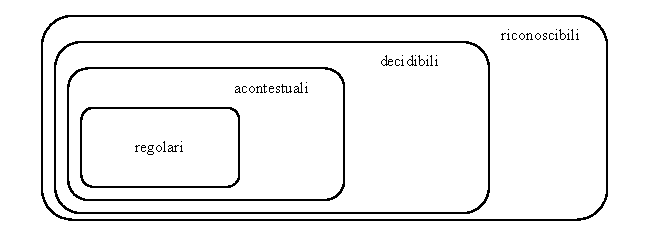
\includegraphics[width=0.7\textwidth ]{images/insiemiLinguaggi.pdf}
\end{center}
\subsection{Macchina di Turing Universale}
Vedremo che il linguaggio contenente le codifiche delle macchine di turing ed una qualsiasi stringa che accettano, è riconoscibile ma non decidibile.
\eqImportante{$ A_{TM}=\{<M,w> \ | \ M\in TM\land w\in L(M)\}$}
\teo{} $A_{TM}$ è turing-riconoscibile.\acc 
\dimo{} Si definisce una TM nota detta \textit{macchina di Turing universale} denotata $U$, sarà quella che riconoscerà $A_{TM}$. Avrà 2 nastri, nel primo conterrà la codifica dell'input $<M,w>$, nel secondo conterrà la configurazione corrente $<(a,q,b)>$ dell'esecuzione simulata di $M$.\acc 
È necessario definire la codifica di $M,w$. Essendo 
$$ M=(Q,\Sigma,\Gamma,\delta,q_0,q_{acc},q_{rej})$$
Siano 
$$ n=|\Sigma| \ \ m=|\Gamma| \ \ s=|Q|$$
la codifica sarà 
$$ (n)_2,(m)_2,(s)_2,<\delta>$$
dove $,$ è un carattere speciale, $(k)_2$ è la codifica binaria di $k\in\Z$ e $<\delta>$ è la codifica binaria delle transizioni 
$$ <\delta>=R_1;R_2\dots;R_j$$
Le regole sono del tipo 
$$ R=((q,a),(r,b,z)) \ \ \ \ z\in\{L,R\}$$
I passi di esecuzione sono i seguenti\begin{enumerate}
    \item Sul nastro 2 viene scritta la configurazione iniziale 
    \item al passo $t$-esimo, la configurazione sarà del tipo $$ <(a,q,b)>$$\begin{enumerate}
        \item si estrae $q$ dalla configurazione 
        \item si scansiona il nastro 1 in cerca di una regola del tipo $$ <(q,x),(r,y,z)>$$
        se $x\ne b[1]$\footnote{primo carattere di $b$}, si controlla la regola successiva, se $x=b[1]$
        si aggiorna la configurazione sul nastro 2 in accordo con la regola letta. 
        \item se il nastro 2 contiene una configurazione con uno stato fra $q_{acc},q_{rej}$, accetta o rifiuta di conseguenza. 
    \end{enumerate}
    \item Se $w\in L(M)$, $U$ accetta, altrimenti rifiuta. Se $M$ va in loop, $U$ andrà in loop di conseguenza. 
\end{enumerate}
$U$ è quindi un riconoscitore per $A_{TM}$.\hfill$\blacksquare$\acc 
\subsection{Diagonalizzazione}
La diagonalizzazione è una tecnica utilizzata per dimostrare alcune semplici proprietà degli insiemi. Sappiamo un insieme generico $A$ è numerabile se esiste una biezione da $\N$ a $A$. Ad esempio, l'insieme dei numeri pari $E$ è numerabile perché esiste $$ f:E\rightarrow \N\ \ \ | \ \ \  f(n)=2n$$ che è una biezione.\acc 
\teo{} $\R$ non è numerabile.\acc 
\dimo{} è necessario dimostrare che un sottoinsieme di $\R$ non sia numerabile. Si pone per assurdo che esiste una biezione da $\N$ a $[0,1]$. Sia $f$ tale biezione, ad ogni valore di $\N$ associa un numero reale fra zero ed uno.$$ \begin{matrix}
    f(1)=0.52423\dots\\ 
    f(2)=0.08362\dots\\ 
    f(3)=0.92841\dots\\ \vdots
\end{matrix}$$
Si definisce un numero $d$ tale che, la parte intera di $d$ è 0, e l'$i$-esima cifra decimale di $d$ è diversa dall'$i$-esima cifra decimale di $f(i)$.\begin{center}
    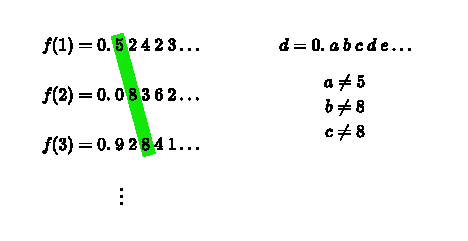
\includegraphics[width=0.7\textwidth ]{images/realiNonNumerabili..pdf}
\end{center}
Essendo $f$ biettiva per ipotesi, $\exists k \in \N | f(k)=d$, ma in questo modo la $k$-esima cifra di $f(k)$ è identica alla $k$-esima cifra di $d$, dato che $d=f(k)$. Ma allora $d$ non è contenuto nell'immagine di $f$, quindi $f$ non è biettiva. \hfill$\blacksquare$\acc 
\prop{} L'insieme delle stringhe binarie (o non) di lunghezza infinita non è numerabile.\acc 
La dimostrazione sarà omessa, ma si può dimostrare con la diagonalizzazione. Si presenteranno ora due proposizioni che saranno utili a dimostrare un risultato fondamentale.\acc 
\prop{1} L'insieme $TM$ di tutte le macchine di turing è numerabile.\acc 
\dimo{1} Si consideri $\Sigma^*$, ossia l'insieme di tutte le stringhe finite (su un generico alfabeto $\Sigma$). Ogni macchina di turing $M$ può essere codificata con una stringa finita. Quindi 
$$ \{<M>\ |\ M\in TM\}\subseteq \Sigma^*$$
Si definisce una relazione d'ordine $<_l$ che rappresenta l'ordinamento lessicografico per tutte le 
stringhe di $l$ caratteri. Si estende poi  a tutte le stringhe con la relazione $<^*$ definita 
$$ x<^*y\iff 
    |x|<|y| \lor (|x|=|y|\land x<_l y)
$$
$<^*$ è una relazione d'ordine totale. Si definisce $f:\N\rightarrow \Sigma^*$ 
$$ f(i)=i\text{-esimo elemento di $\Sigma^*$ secondo l'ordinamento }<^*$$
$f$ è una biezione dato che per ogni $i\in\N$ si può associare un elemento di $\Sigma^*$. Quindi $\Sigma^*$ è numerabile, e di conseguenza $\{<M>\ |\ M\in TM\}$ è numerabile. \hfill$\blacksquare$\acc 
\prop{2} L'insieme dei linguaggi non è numerabile.\acc 
\dimo{2} Sia $\mathcal{L}$ l'insieme di tutti i linguaggi le cui stringhe sono binarie. Un generico linguaggio $L$ è in $\Sigma^*$ dove $\Sigma=\{0,1\}$. 
Definisco per ogni linguaggio $L$ una stringa binaria $\mathcal{X}_L$ di lunghezza infinita tale che 
\begin{center}
    l'$i$-esimo carattere di $\mathcal{X}_L$ è 1 se l'$i$-esimo elemento di $\Sigma^*$ (secondo un arbitrario ordinamento) è in $L$. Altrimenti è 0. 
\end{center}
Questa applicazione $f:\mathcal{L}\rightarrow\mathcal{B}$ è biettiva, $\mathcal{B}$ è l'insieme delle stringhe di lunghezza infinita, che sappiamo non essere numerabile, ma allora anche $\mathcal{L}$, ossia un sotto-insieme del totale dei linguaggi non è numerabile, implica che l'insieme dei linguaggi non è numerabile. \hfill$\blacksquare$\acc 
\teo{ fondamentale } Esistono linguaggi che non sono turing riconoscibili. \acc 
\dimo{} Ogni macchina di turing ha ad esso associato un solo linguaggio. Essendo l'insieme dei linguaggi non numerabile, ed essendo l'insieme delle TM numerabile, esiste almeno un linguaggio che non si può associare a nessuna TM $\implies$ esistono linguaggi non riconoscibili.\hfill$\blacksquare$\acc 
\teo{} $A_{TM}$ \textbf{non} è turing-decidibile.\acc 
\dimo{} Si utilizzerà la diagonalizzazione. Si pone per assurdo che esiste una TM $H$ che è un decisore per $A_{TM}$, ovvero 
$$ H(<M,w>)=\begin{cases}
    \text{accetta se $M$ accetta $w$}\\ 
    \text{rifiuta se $M$ rifiuta $w$}
\end{cases}$$
Si definisce una nuova TM $D$ che prende come input una TM e si comporta nel seguente modo \begin{enumerate}
    \item Su input $<M>$, esegue $H(<M,<M>>)$
    \item Se $H$ accetta, $D$ rifiuta. Se $H$ rifiuta, $D$ accetta.
\end{enumerate}
Ricordando il comportamento di $H$, si ha la seguente situazione "transitiva"
\begin{center}
    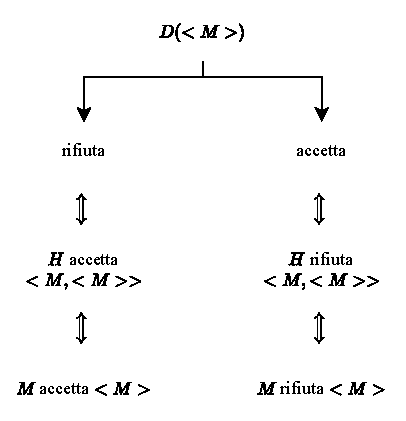
\includegraphics[width=0.6\textwidth ]{images/ATMnonDec.pdf}
\end{center}
Se alla TM $D$ si da in input $<D>$ si ricade nella seguente situazione.
\begin{center}
    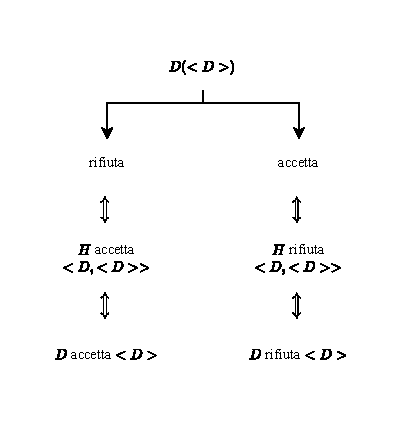
\includegraphics[width=0.6\textwidth ]{images/ATMnonDec2.pdf}
\end{center}
Ma allora $D$ accetta $<D>$ solo e soltanto se $D$ rifiuta $<D>$. È una palese contraddizione, è quindi impossibile che $H$ sia un decisore per $A_{TM}$.
\hfill$\blacksquare$\acc 
\defi{(co-turing Riconoscibilità)} $L$ è co-turing riconoscibile (o più semplicemente, co-riconoscibile) se $\overline{L}$ è turing riconoscibile.\acc 
\teo{} $L$ è decidibile se e solo se $L$ è sia riconoscibile che co-riconoscibile.\acc 
\dimo{} Si dimostrano separatamente le due implicazioni. \\ 
\boxedMath{$\implies$} Per ipotesi $L$ è decidibile, allora anche $\overline{L}$ lo è, quindi sia $L$ che $\overline{L}$ sono riconoscibili. \\ 
\boxedMath{$\impliedby$} Per ipotesi $L$ ed $\overline{L}$ sono riconoscibili. Siano $M_1,M_2$ le TM che li riconoscono. Si costruisce una nuova TM $M$ tale che \begin{enumerate}
    \item su input $w$ esegue parallelamente $w$ su $M_1$ ed $M_2$
    \item se $M_1$ accetta, $M$ accetta. se $M_2$ accetta, $M$ rifiuta.
\end{enumerate}
$\forall w$ si ha che $w\in L \lor w\in \overline{L}$, solamente una fra $M_1,M_2$ può accettare $w$, quindi $M$ non può mai andare in loop $\implies$ $M$ è un decisore per $L$.\hfill$\blacksquare$\acc 
\textbf{Corollario} : $\overline{A_{TM}}$ non è turing riconoscibile.\flowerLine 
\section{Riducibilità}
La riducibilità è una tecnica che permette di dimostrare la non decidibilità/non riconoscibilità di molti linguaggi. Informalmente, dati due linguaggi $A$ e $B$,  diremo che $A$ \textbf{si riduce a} $B$, e denoteremo $$ A\le B$$ Se esiste un algoritmo (una TM) per $B$ che risolve (decide) anche $A$.\begin{quotation}
    trovare una soluzione per $A$ \textbf{non può essere} più difficile di trovare una soluzione per $B$
\end{quotation}
Si consideri il seguente linguaggio 
$$ HALT_{TM}=\{<M,w> \ | \ M\in TM\land M(w)\text{ termina} \}$$
Data una TM si deve stabilire se termina o continua all'infinito su un certo input.\acc 
\teo{(Halting Problem)} $HALT_{TM}$ non è decidibile.\acc 
\dimo{} Per assurdo, sia $R$ un decisore per $HALT_{TM}$. Si definisce una TM $S$ tale che \begin{enumerate}
    \item prende come input una TM ed una stringa $<M,w>\in A_{TM}$
    \item esegue $R$ su $<M,w>$
    \item se $R$ accetta (quindi si ha la certezza che $M$ termina), $S$ simula $M$ su $w$ ed accetta solamente se $M$ accetta $w$.
\end{enumerate}
Quindi $S$ è un decisore per tutte le coppie $<M,w>$ ossia $A_{TM}$. Ma $A_{TM}$ non è decidibile, è quindi impossibile che esista un decisore per $HALT_{TM}$.\hfill$\blacksquare$\acc 
Si consideri 
$$ E_{TM}=\{<M>\ | \ M\in DFA \land L(M)=\emptyset\}$$
\prop{} $E_{TM}$ non è decidibile.\acc 
\dimo{} Si pone per assurdo che $R$ decide $E_{TM}$. Si definisce una nuova TM $S$ che prende come input gli elementi di $A_{TM}$ e si comporta come segue \begin{enumerate}
    \item costruisce una nuova TM $M'$, il cui comportamento è il seguente\begin{enumerate}
        \item prende come input una stringa $x$
        \item se $x\ne w$ rifiuta 
        \item se $x=w$ esegue $M$ su input $w$
        \item $M'$ accetta se $M$ accetta
    \end{enumerate}
    \item esegue $R$ su input $<M'>$
    \item se $R$ accetta, $S$ rifiuta. Se $R$ rifiuta, $S$ accetta.
\end{enumerate}
Essendo $R$ un decisore, allora $S$ è un decisore di $A_{TM}$, ma $A_{TM}$ non è decidibile, è quindi impossibile che esista un decisore per $E_{TM}$.\hfill$\blacksquare$\acc 
Si vuole formalizzare il concetto di riduzione, intuitivamente si può dire che la riduzione è definita da una funzione, che negli obiettivi di questo corso sarà calcolata da una TM.\acc 
\defi{} Una funzione $f:\Sigma^*\rightarrow \Sigma^*$ si dice \textbf{calcolabile} se esiste una TM che su input $w$ termina scrivendo sul nastro $f(w)$. Spesso tale TM ha un nastro dedicato per l'output della funzione.\acc 
Nell'halting problem è stata definita una TM a tal scopo. La definizione di riduzione che verrà data non rappresenta il concetto in senso lato, bensì è la sua formulazione più semplice detta \textit{mapping reduction}, sufficiente per gli obiettivi di questo corso.\acc 
\defi{(Riduzione)} Siano $A$ e $B$ due generici linguaggi. Si dice che $A$ è \textbf{riducibile} a $B$, e si denota 
$$ A\le_m B$$
Se \textit{esiste} una funzione calcolabile $f:\Sigma^*\rightarrow \Sigma^*$ tale che 
$$ \forall w\in\Sigma^*, \ \ w\in A \iff f(w)\in B$$
Il seguente teorema è di fondamentale importanza quando si vuole dimostrare la non decidibilità di un linguaggio.\acc 
\teo{} Se $A\le_m B$ e $B$ è decidibile, allora  anche $A$ è decidibile.\acc 
\dimo{} Sia $M_B$ un decisore per $B$, si definisce una TM $A_M$ tale che \begin{enumerate}
    \item su input $w\in\Sigma^*$, calcola $f(w)$
    \item esegue $M_B$ su input $f(w)$ 
    \item Se $M_B(f(w))$ accetta, $M_A$ accetta, altrimenti rifiuta.
\end{enumerate}
Essendo che, per ogni $w$ si ha che $w\in A$ solo se $f(w)\in B$, $M_A$ potrà sempre o accettare o rifiutare (data l'ipotesi che $M_B$ è un decisore), quindi  $M_A$ è un decisore per $A$.
\hfill$\blacksquare$\acc 
\textbf{Corollario} : Se $A\le_m B$ e $A$ non è decidibile, allora  anche $B$ non è decidibile.
\subsection{Applicazioni della Riducibilità}
In questa sezione verranno trattati differenti esempi di come la \textit{riducibilità} può essere usata per dimostrare la non decidibilità di molti linguaggi, e verranno presentati \textit{alcuni risultati} che estendono le applicazioni, in particolare, quando si trattano linguaggi non riconoscibili. È \underline{consigliato} allo studente che deve sostenere l'esame di porre particolare attenzione a questa sezione.
\esempio{1}
Si vuole dimostrare in maniera formale l'indecidibilità di $HALT_{TM}$. La notazione $M(w)\ne\infty$ indicia che la TM $M$ su input $w$ non va in loop, e termina. 
$$ HALT_{TM}=\{<M,w> \ | \ M\in TM\land M(w)\ne\infty \}$$
Basta dimostrare che $$ A_{TM}\le_m HALT_{TM}$$
Essendo $A_{TM}$ indecidibile, ciò comporterebbe anche l'indecidibilità di $HALT_{TM}$. Si definisce una funzione $\ridFunc$ tale che 
$$ \forall <M,w>\in\Sigma^*, \ \ \ <M,w>\in A_{TM}\iff f(<M,w>)\in HALT_{TM}$$
$f$ deve essere calcolabile, quindi si definisce una TM che calcola $f$, ed esegue i seguenti passi 
\begin{enumerate}
    \item Su input $<M,w>$ costruisce una TM ausiliaria $M'$
    \item Tale $M'$ su un generico input $x$, esegue i seguenti passi\begin{enumerate}
        \item Esegue $M$ su input $x$
        \item Se $M(x)$ accetta, allora $M'$ rifiuta, se $M(x)$ rifiuta, entra volontariamente in uno stato di loop.
    \end{enumerate}
    \item L'output della funzione sarà $<M',w>$
\end{enumerate}
\boxedMath{$\implies$} se $<M,w>\in A_{TM}$, allora $M$ accetta $w$, pertanto $M'$ a sua volta accetterà $w$, terminando. Si ha quindi che $<M',w>\in HALT_{TM}$. La prima implicazione della riducibilità è dimostrata. \acc 
\boxedMath{$\impliedby$} se $<M,w>\notin A_{TM}$, allora $M(w)$ o rifiuta, o va in loop. \begin{itemize}
    \item Se $M(w)$ rifiuta, per definizione, $M'$ entra in uno stato di loop. 
    \item Se $M(w)$ va in loop, anche $M'$ (che la esegue) va in loop.
\end{itemize}
Si ha quindi che, se  $<M,w>\notin A_{TM}$, la TM $M'$ va in loop su $w$, quindi non termina, allora 
$$f(<M,w>)=<M',w>\notin HALT_{TM}$$La seconda implicazione della riducibilità è dimostrata. Quindi 
$ A_{TM}\le_m HALT_{TM}$. Ne consegue che $HALT_{TM}$ è indecidibile.
\esempio{2}
Si vuole dimostrare l'indecidibilità di $EQ_{TM}$. 
$$ EQ_{TM}=\{<M_1,M_2> \ | \ M_1,M_2\in TM\land L(M_1)=L(M_2) \}$$
Basta dimostrare che $$ E_{TM}\le_m  EQ_{TM}$$Si definisce una funzione $\ridFunc$ tale che 
$$ \forall <M>\in\Sigma^*, \ \ \ <M>\in E_{TM}\iff f(<M>)\in EQ_{TM}$$
$f$ deve essere calcolabile, quindi si definisce una TM che calcola $f$, ed esegue i seguenti passi 
\begin{enumerate}
    \item   Su input $<M>$, definisce una TM ausiliaria $M'$, la cui computazione è descritta come segue \begin{enumerate}
        \item $M'$ su un qualsiasi input $x$ rifiuta sempre.
    \end{enumerate}
    \item L'output della funzione sarà $<M,M'>$
\end{enumerate}
\boxedMath{$\implies$} Se $M\in E_{TM}$, allora $L(M)=\emptyset$. Essendo che $M'$ rifiuta su ogni input, anche il suo linguaggio è vuoto, quindi $L(M)=L(M')$, ne consegue che $<M,M'>\in EQ_{TM}$.
\acc \boxedMath{$\impliedby$} Se $M\notin E_{TM}$, allora $L(M)\ne \emptyset$, Essendo che $M'$ rifiuta su ogni input, il suo linguaggio è vuoto, quindi $L(M)\ne L(M') = \emptyset$, ne consegue che $<M,M'>\notin EQ_{TM}$.\acc 
Risulta naturale chiedersi: È possibile utilizzare la riducibilità per dimostrare anche la non riconoscibilità di un linguaggio? Il seguente teorema risponde a tale domanda. \acc 
\teo{} Se $A\le_m B$ e $B$ è riconoscibile, allora  anche $A$ è riconoscibile.\acc 
\textbf{Corollario} : Se $A\le_m B$ e $A$ non è riconoscibile, allora  anche $B$ non è riconoscibile.\acc 
Essendo che $A_{TM}$ è riconoscibile ma non decidibile, per il teorema sulla co-riconoscibilità è noto che il linguaggio $\overline{A_{TM}}$ non è riconoscibile. È possibile utilizzare $\overline{A_{TM}}$ e la riducibilità per dimostrare la non riconoscibilità di molti linguaggi. $\overline{A_{TM}}$  è però un linguaggio ambiguo con la quale lavorare, risulta più funzionale considerare direttamente $A_{TM}$ grazie al seguente teorema.\acc 
\teo{} Se $A\le_m B$, allora $\overline A\le_m \overline B$.\acc 
\dimo{} La funzione $f$ rimane invariata dato che $ \forall w\in\Sigma^*$ si ha che $$\begin{matrix}
    w\in A\iff f(w)\in B \\ \\ 
    w\in \overline A\iff f(w)\in \overline B 
\end{matrix} $$\hfill$\blacksquare$\acc 
Le conseguenze sono ovvie, se $A\le_m B$ e $\overline A$ non è riconoscibile, allora anche $\overline B$ non è riconoscibile. Per dimostrare la non riconoscibilità di un generico linguaggio $A$, basterà dimostrare $A_{TM}$ si riduce a $\overline A$.
\esempio{3}
Si vuole dimostrare la non riconoscibilità di ${EQ_{TM}}$. 
Basta dimostrare che $$ A_{TM}\le_m  \overline{EQ_{TM}}$$Si definisce una funzione $\ridFunc$ tale che 
$$ \forall <M,w>\in\Sigma^*, \ \ \  <M,w>\in A_{TM}\iff f( <M,w>)\in \overline{EQ_{TM}}$$
In pratica, se $M$ accetta $w$, allora $f(<M,w>)$ deve restituire due TM che hanno linguaggi differenti.  
$f$ deve essere calcolabile, quindi si definisce una TM che calcola $f$, ed esegue i seguenti passi 
\begin{enumerate}
    \item  Su input $<M,w>$, definisce due TM ausiliarie $M_1,M_2$, tali che \begin{itemize}
        \item $M_1$ rifiuta sempre 
        \item $M_2$ accetta solo se $M(w)$ accetta, altrimenti rifiuta.
    \end{itemize}
    \item l'output della funzione è $<M_1,M_2>$
\end{enumerate}
\boxedMath{$\implies$} Se $<M,w>\in A_{TM}$, essendo che $M(w)$ accetta si ha che \begin{itemize}
    \item $M_1$ rifiuta sempre 
    \item  $M_2$ accetta sempre 
\end{itemize}
Quindi $L(M_1)\ne L(M_2)\implies <M_1,M_2>\in  \overline{EQ_{TM}}$.
\acc \boxedMath{$\impliedby$} Se $<M,w>\notin A_{TM}$, essendo che $M(w)$ rifiuta si ha che \begin{itemize}
    \item $M_1$ rifiuta sempre 
    \item  $M_2$ rifiuta sempre 
\end{itemize}
Quindi $L(M_1)=L(M_2)=\emptyset \implies <M_1,M_2>\in  {EQ_{TM}}\implies <M_1,M_2>\notin  \overline{EQ_{TM}}$. Ne consegue che $EQ_{TM}$ non è riconoscibile.
\esempio{4}
Si vuole dimostrare la non decidibilità di $L$ definito come segue 
$$ L=\{<M>\ | \ M\in TM \land w\in L(M)\implies w\in \{0,1\}^*\land |w|\%2=1\}$$ 
Ossia il linguaggio di tutte le TM che accettano esclusivamente stringhe binarie di lunghezza dispari.
Basta dimostrare che $$ A_{TM}\le_m  L$$Si definisce una funzione $\ridFunc$ tale che 
$$ \forall <M,w>\in\Sigma^*, \ \ \  <M,w>\in A_{TM}\iff f( <M,w>)\in L$$
$f$ deve essere calcolabile, quindi si definisce una TM che calcola $f$, ed esegue i seguenti passi 
\begin{enumerate}
    \item  Su input $<M,w>$, definisce una TM ausiliaria $M'$, tale che:
    \item Su input $x$, se $|x|\%2=0$ rifiuta. 
    \item Altrimenti, accetta se e solo se $M$ accetta $w$.
    \item L'output sarà $M'$.
\end{enumerate}
\boxedMath{$\implies$} Se $<M,w>\in A_{TM}$, essendo che $M(w)$ accetta si ha che 
$M'$ accetterà tutte e sole le stringhe binarie di lunghezza dispari, quindi $f(<M,w>)=M'\in L$.
\acc \boxedMath{$\impliedby$} Se $<M,w>\notin A_{TM}$, $M'$ rifiuterà a prescindere, si avrà che 
$L(M')=\emptyset\implies M'\notin L$. Ne consegue che $L$ è indecidibile.
\esempio{5}
Si vuole dimostrare la non decidibilità di $L$ definito come segue 
$$ L=\{<M>\ | \ M\in TM \land L(M)=\{0^n1^n0^n,\ n\ge 0\}\}$$ 
Basta dimostrare che $$ A_{TM}\le_m  L$$Si definisce una funzione $\ridFunc$ tale che 
$$ \forall <M,w>\in\Sigma^*, \ \ \  <M,w>\in A_{TM}\iff f( <M,w>)\in L$$
$f$ deve essere calcolabile, quindi si definisce una TM che calcola $f$, ed esegue i seguenti passi 
\begin{enumerate}
    \item  Su input $<M,w>$, definisce una TM ausiliaria $M'$, tale che:
    \item Su input $x$, esegue $M(w)$. 
    \item Se $M(w)$ accetta, $M'$ accetta solo se $x\in\{0^n1^n0^n,\ n\ge 0\}$, altrimenti rifiuta.
    \item Se $M(w)$ rifiuta, $M'$ rifiuta a prescindere. 
    \item L'output sarà $M'$.
\end{enumerate}
\boxedMath{$\implies$} Se $<M,w>\in A_{TM}$, essendo che $M(w)$ accetta si ha che 
$M'$ accetterà solo se $$x\in\{0^n1^n0^n,\ n\ge 0\}$$quindi $L(M')=\{0^n1^n0^n,\ n\ge 0\} \implies f(<M,w>)=M'\in L$.
\acc \boxedMath{$\impliedby$} Se $<M,w>\notin A_{TM}$, $M'$ rifiuterà a prescindere (o andrà in loop nel caso $M(w)$ vada in loop), si avrà che 
$L(M')=\emptyset\ne \{0^n1^n0^n,\ n\ge 0\} \implies M'\notin L$. Ne consegue che $L$ è indecidibile.
\esempio{6}
Si vuole dimostrare la non decidibilità di $L$ definito come segue 
$$ L=\{<M>\ | \ M\in TM \land L(M)\supseteq \{w\ | \ w\text{ inizia con uno }0\}\}$$ 
Ossia il linguaggio di tutte le TM il cui linguaggio contiene ogni stringa che inizia con 0.
Basta dimostrare che $$ A_{TM}\le_m  L$$Si definisce una funzione $\ridFunc$ tale che 
$$ \forall <M,w>\in\Sigma^*, \ \ \  <M,w>\in A_{TM}\iff f( <M,w>)\in L$$
$f$ deve essere calcolabile, quindi si definisce una TM che calcola $f$, ed esegue i seguenti passi 
\begin{enumerate}
    \item  Su input $<M,w>$, definisce una TM ausiliaria $M'$, tale che:
    \item su ogni input $x$ esegue $M(w)$, e se questa accetta, $M'$ accetta, altrimenti rifiuta.
    \item L'output sarà $M'$.
\end{enumerate}
\boxedMath{$\implies$} Se $<M,w>\in A_{TM}$, essendo che $M(w)$ accetta si ha che 
$M'$ accetterà ogni input, quindi $L(M')=\Sigma^*$ ed essendo l'insieme di ogni stringa, conterrà anche ogni stringa che inizia con zero, allora $<M'>\in L$.
\acc \boxedMath{$\impliedby$} Se $<M,w>\notin A_{TM}$, $M'$ rifiuterà  (o andrà in loop nel caso $M(w)$ vada in loop), si avrà che 
$L(M')=\emptyset$, quindi non conterrà nemmeno una stringa che inizia con 0, allora  $<M'>\notin L$.
Ne consegue che $L$ è indecidibile.
\esempio{7}
Si vuole dimostrare la non decidibilità di $U$ definito come segue 
$$ U=\{<T,T'> \| \ T,T'\in TM\land L(T)\cup L(T')=\Sigma^*\}$$ 
Ossia il linguaggio di tutte le coppie di TM la cui unione dei linguaggi equivale all'insieme di tutte le stringhe.
Basta dimostrare che $$ A_{TM}\le_m  U$$Si definisce una funzione $\ridFunc$ tale che 
$$ \forall <M,w>\in\Sigma^*, \ \ \  <M,w>\in A_{TM}\iff f( <M,w>)\in U$$
$f$ deve essere calcolabile, quindi si definisce una TM che calcola $f$, ed esegue i seguenti passi 
\begin{enumerate}
    \item  Su input $<M,w>$, definisce una TM ausiliaria $T$ che rifiuta per ogni input $x$. 
    \item Definisce poi una TM $T'$ che accetta solo se $M(w)$ accetta. 
    \item L'output è $<T,T'>$
\end{enumerate}
\boxedMath{$\implies$} Se $<M,w>\in A_{TM}$, essendo che $M(w)$ accetta si ha che
$T'$ accetterà ogni stringa ed il suo linguaggio sarà uguale a tutte le stringhe. $T$ invece avrà linguaggio vuoto. $L(T)\cup L(T')=\emptyset\cup \Sigma^*=\Sigma^*\implies <T,T'>\in U$.
\acc \boxedMath{$\impliedby$} Se $<M,w>\notin A_{TM}$, $M'$ rifiuterà  (o andrà in loop nel caso $M(w)$ vada in loop), si avrà che 
$L(T')=\emptyset$, inoltre anche $T$ ha linguaggio vuoto, quindi $L(T)\cup L(T')=\emptyset\ne \Sigma^*\implies <T,T'>\notin U$. Ne consegue che $U$ è indecidibile.
\end{document}